\chapter{Time-Invariant Model of ATS}\label{ch:tim_ats}
This chapter focuses on tackling the main problems for an ATS. First, a time-invariant vehicle-centric model for the transportation network is developed in \secref{sec:vc_model}. The model presented in this document expands upon the one formulated in \cite{project_thesis}, using graph theory and a vehicle-centric approach to provide flexibility in handling different vehicle capacities and types. This model be the basis upon which sub-problems of an ATS will be formulated and analyzed in \secref{sec:ats_challenges_analysis}. With those hinsights, the Complete ATS Managing problem will be formulated in \secref{sec:catsm} and its performance evaluated in \secref{sec:use_case_analysis_ats}. 
\section{Vehicle-centric Model}\label{sec:vc_model}
The model provided in this section will expand the model formulated in \cite{project_thesis}. It is worth noting that, although the model presented in \cite{project_thesis} is specific for the scenario described in the same work, it can be expanded to cover more general use cases.
Therefore, the model of the transportation network will be developed using graph theory. While much of the existing literature relies on fluid-dynamic models (\cite{amod_review}), wherein customers and AVs are depicted as continuous flows between nodes, this study will employ a combination with a vehicle-centric approach. In the latter, customers and AVs will be individually modeled. Contrary to the solutions proposed by most of the literature, this work combines mobility of people with goods transportation, therefore modeling vehicles individually will provided the required flexibility to handle different capacities and the increased complexity given by the plethora and variety of vehicles, the set of which will be indicated as $\mathcal{A}$.  \\ 
Let $\mathcal{G} = \langle \mathcal{V}, \mathcal{E} \rangle$ being the directed graph representing corresponding transportation network of a city, where $\mathcal{V}$ is the set of vertices and $\mathcal{E} \subseteq \mathcal{V} \times \mathcal{V}$ is the set of edges. Any vertex, or node,  $ v \in  \mathcal{V}$ represents a location. For the context of this paper, the two terms will be used intercheangeably, as they ultimately indicate the same thing. Following the work in \cite{project_thesis}, each node consists of an area of interests. An edge $\langle v_i, v_j \rangle \in \mathcal{E}$ represents a connection, which can consist of a road or a combination of those, linking $v_i$ to $v_j$. The level of abstraction is decided by the engineer and can be used to regulate the granularity of the model. Locations $v_i$ and $v_j$ can indicate low level key points, such as cross roads or trafficated traffic lights, as well as higher level areas such as residental areas or leisure centers. Similarly, an edge can contain multiple crossroads or joints or simply indicating a path from $v_i$ to $v_j$, regardless of additional details. A correct granularity is not trivial to decide a priori and a general approach is likewise hard to delineate.  Determining the level of abstraction remains, therefore, an engineer's prerogative and highly depends on the system in question. It is also worth noting that the, for conveniency and to better reflect the situation in real world applications, the graph is a uni-direct graph. To model a two-way road, one should simply make use of two edges from locations $v_i$ and $v_j$. \\
As also described in \cite{project_thesis}, each edge is associated with multiple metrics and information. \\
Firstly, at each edge one must attribute a travel time $T$. $T$ is a function $T: \mathcal{E} \times \mathcal{A} \rightarrow \mathbb{R}_{> 0}$, which at each given a vehicle and edge maps a float value $T_{i,j}^a \in \mathbb{R}_{\geq 0}$ indicating the time required for the  vehicle of type $a$ to travel the path from $v_i$ to $v_j$. In this work, the unit of  $T_{i.j}^a$ is not of particular interest, as it depends on the application. \\
Secondly, each edge is also associated with a distance $d: \mathcal{E} \rightarrow \mathbb{R}_{\geq 0}$, which maps an edge to a float value $d_{i,j}$ indicating the distance from $v_i$ to $v_j$. \\
Another factor which is considered in this work, as stated above, is pollution. This metric is associated to each edge and is a function 
$f: \mathcal{E} \times \mathcal{A} \rightarrow \mathbb{R}_{\geq 0}$. To simplify the discussion for this work, $f$ is assumed to produce a certain value refered to as pollution index. In other words, it is not supposed to represent a measurable element, such as $\text{CO}_2$ emissions, but rather a value which can represent multiple quantitative factors and is higher if the combination of path and vehicle type is highly polluting. While it can be argued that the pollution can also be simply a function of $d$ and $T$, this abstraction does not account for other elements, such as road type, vehicle fuel and road slope. The index $f$, therefore, is a mathematical abstraction which allows a more flexible model for the system. To use this abstraction, however, each edge must include additional information, including the one mentioned before. \\
Similarly to what observed by \citepaperofs{congestion_vrp_phd_graph}{Zhang}, we can introduce the concept of congestions in the model by constraining the routing by the capacity of each road. In other words, we can associate each edge with a capacity $c: \mathcal{E} \rightarrow \mathbb{N}_{> 0}$ indicating the limit in terms of car occupancy above which the traffic in that edge slows down eventually reaching a congestion. As pointed out in \cite{congestion_vrp_phd_graph}, this semplified model is adequate in this context as well as the aim of this work focusing solely on the control of vehicles to prevent congestion rather than analyzing their behavior in congested network. While it is understood that congestions behave differently in real world scenarios and other, more sophisticated approaches exist (\cite{lindsey1999congestion}, \cite{verhoef1999time}), for the sake of simplicity, we will assume $T_{ija} = \infty $ if the number of vehicles in that edge from  $\langle v_i, v_j \rangle$ to be larger than the capacity $c_{ij}$.\\
In addition, each edge $\langle v_i, v_j \rangle$ will also include information regarding traffic limitations, i.e. whether a vehicle type is allowed or not to travel that link. Intuitively, limitations will be represented as a function $s: \mathcal{E} \times \mathcal{A} \rightarrow\{0,1\}$, where $1$ implies the vehicle can traver that edge. Following the example in \cite{project_thesis}, limitations can be because of various factors, like for e.g. weight or height. For this reason, it is convenient to abstract away such details and just indicate wether a link is can be traversed or not. Notably, one could use this representation to transform a bidirect graph $G'$ to be equivalent to $G$ by letting $s(e,a) = 0$ for any one-way road $e = \langle v_i, v_j \rangle$ for all $a \in \mathcal{A}$. For convenience, this function will be incorporated in the definition of the capacity, updating it to become \equaref{eq:capacity}. 
\begin{equation}
	c(e = \langle v_i, v_j \rangle) = 
	\begin{cases}
		0 & \text{if } s(e) = 0 \\
		c(e) & \text{otherwise}
	\end{cases}
	\label{eq:capacity}
\end{equation}
Following the discussion above, this is equivalent to setting $T_{ija} = \infty$ for all $a \in \mathcal{A}$ according to this model specifications. In this way, we can treat the road as being unaccessible without increasing the number of conditions and decrease the redeability of the model. \\
As mentioned above, the set of autonomous vehicles is indicated as $\mathcal{A}$ and each vehicle will be modeled as a tuple $\langle \underline{s_a},\bar{t_a}, S_a, Q_a, I^b_a, R^-_a, R^+_a, \theta_a, B_a(t),\mathcal{R}_a, \mathcal{T}_a \rangle$. $\underline{s_a}\in \mathcal{V} \text{ and } \bar{t_a}\in \mathcal{V}$ are the starting and terminal node respectively; $Q_a \in \mathbb{R}_{>0}$ will be used to indicate battery capacity and charing rate and discharging rate will be represented as  $R^+_a \in \mathbb{R}_{>0}\text{ and } R^-_a\in \mathbb{R}_{>0}$ respectively; $\theta_a \in [0,1]$ is used to model the battery breakpoint and $B_a(t)\in \mathbb{R}_{\ge0}$ is the state of charge at time $t$; $\mathcal{R}_a$ is the set of requests assigned to vehicle $a$ and $\mathcal{T}_a$ is the type. For a more detailed understanding of the vehicle type, the reader is encouraged to analyze the discussion in \cite{project_thesis}. For the purpose of this work, the vehicle type will be understood as a tuple $\langle P_a, G_a, C_a, F_a \rangle$, where , $G_a \in \mathbb{R}_{\ge0}$ and $P_a \in \mathbb{R}_{\ge0}$
are the goods and people capacity and $C_a \in \mathbb{R}_{>0}$ and $F_a \in \mathbb{R}_{>0}$ indicate operational cost and pollution factor respectively. Furthermore, each set of assigned requests $\mathcal{R}_a$ is a subset of the set of all requests in the systems, i.e. $\mathcal{R}_a \subseteq\mathcal{R}$. For the purpose of this model, we will assume each request assignment to be unique, i.e. $\mathcal{R}_a \neq \mathcal{R}_b \text{ and } \mathcal{R}_a \subseteq \mathcal{R} \setminus \mathcal{R}_b,  \text{ for all } (a,b) \in \mathcal{A} \text{ with } a\neq b$. \\
The battery will be modeled according to the two operating mode, i.e. charging and discharging. While it is understood that these two operations are highly influenced by multiple factors, it is sensible to make assumptions in order to simplify the model. 
As it is also widely spread in industry, one can neglet the influence of external factors such as weather condition or intrinsic characteristics of the battery, such as temperature or age. The charging profile will be modelled taking inspiration from the model proposed by \citepaperofs{lee2020model}{Lee}. As mentioned above, the vehicles have a charging rate, a battery capacity and a breakpoint, namely $R^+_a, Q_a \text{ and } \theta_a$ respectively. The state of charge at time $t \in \mathbb{R}_{\ge0}$ of a certain vehicle will be obtained according to the model described in \equaref{eq:cc_cv}, which is derived from the CC-CV (Constant current - Constant Voltage ) scheme. (A more complete explanation can be found in \cite{LIU2020101342}).%$B :\mathbb{R}_{\ge 0} \times \mathcal{A}  \rightarrow \mathbb{R}_{\ge0}$

\begin{figure}[ht]
	\centering
	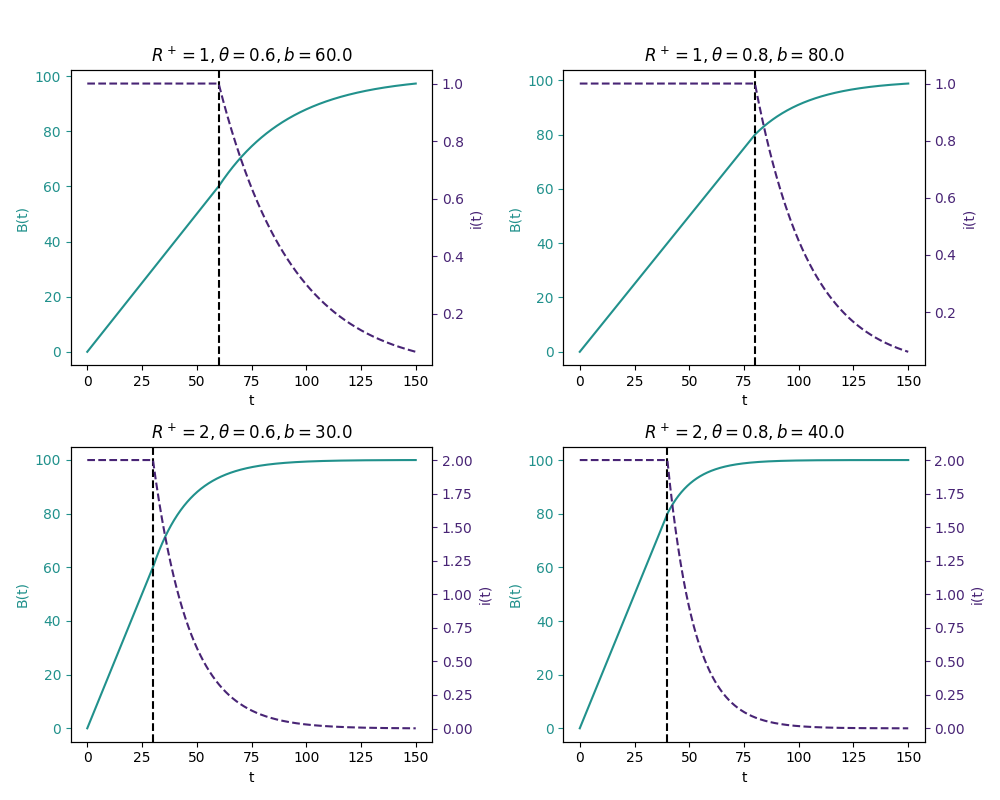
\includegraphics[width =12.5cm]{assets/img/07_graph_based/R_theta_combinations.png}
	\caption[Different Charging Profiles According To The Model]
	{Different charging profile obtained according to the model developed in \equaref{eq:cc_cv}. B is the State of Charge in Percentage, while $i(t)$ in function of the time unit $t$. The battery have $Q = 100$ %and the breakpoint is calculated as $b = \dfrac{Q\theta}{R^+}$  
	}
	\label{fig:charging_profiles}
\end{figure}
\begin{equation}
	B_a(t+1) = 
	\begin{cases} 
		%0 & \text{if } t+1 \leq 0 \\
		%B(t)_a + \int_{t}^{t+1} i(t)dt & \quad \text{if } t \leq  b_a\\
		B(t)_a + R^+_a & \quad \text{if } t \leq  b_a\\
		\\
		%R^+_a e^{-t+b_a} %& \text{else}
		Q_a - \dfrac{Q_ai(t)(1-\theta_a)}{R^+_a}
		\end{cases}
		\label{eq:cc_cv}
\end{equation}

with $b_a = \dfrac{\theta_a Q_a}{R^+_a}$,  $i(t)= \begin{cases} R^+_a \quad \text{if } t \leq  b_a\\
	R^+_a e^{-(t-b_a)/\tau}\\ \end{cases}$ and $\tau= \dfrac{C_n}{R^+_a\theta_a}\in \mathbb{R}_{\ge0}$  representing how quickly the current decreases. The value of $C_n$ depends on the charging device considered.   \\
	An example of the charging profiles from this model can be seen in \figref{fig:charging_profiles}. 
	 Since $i(t)$ is assumed to be constant at time $t\leq b_a$, i.e. $i(t) = R^+_a$,the first condition is derived as follows. 
\begin{align*}
	B_a(t+\alpha) &= B_a(t) + \int_{t}^{t+\alpha}R^+_adt\\
	B_a(t+\alpha) &= B_a(t) +R^+_a \int_{t}^{t+\alpha}dt\\
	B_a(t+\alpha) &= B_a(t) +R^+_a \quad t \bigg|_{t}^{t+\alpha}\\
	B_a(t+\alpha) &= B_a(t) +R^+_a (t+\alpha - t)\\
	B_a(t+\alpha) &= B_a(t) +\alpha R^+_a\\
\end{align*}
with $\alpha = 1$. \\
The discharging, on the other hand, will be modeled as it being directly proportional to the travel time $T$, as described in \equaref{eq:discharging}. 
%\begin{equation}
%	B_a(t+1) = B(t)_a - R^-_a ( \gamma d_a + (1-\gamma)T_a)
%	\label{eq:discharging}
%\end{equation} 
%where $\gamma \in [0,1]$. \\
\begin{equation}
	B_a(t+T_{u,v}^a) = B(t)_a - R^-_a T_{u,v}^a
	\label{eq:discharging}
\end{equation} 
The equation describes the relationship between the initial and final battery levels on edge $\langle v_u, v_v \rangle$ during the transit. Following \equaref{eq:discharging}, one can assign to each edge a rate of battery discharge by defining it as the difference between the state of charge at time $t$ and at time $t+T_{u,v}^a$. \\
\begin{equation}
	 e^a_{u,v} = B(t)_a - B_a(t+T_{u,v}^a) =  R^-_a T_{u,v}^a
	\label{eq:discharging_rate_per_edge}
\end{equation} 
\equaref{eq:discharging_rate_per_edge} allows to describe the discharging rate as a function of only the edge and the vehicle. \\
In terms of operational costs, multiple factors should be considered and the analysis must be extended from the one developed in \cite{project_thesis}, where the operational cost was only in function of the vehicle type. Similarly to the aforementioned work, this model assumes a certain operational cost depending on the vehicle type, however the discussion is also extended in terms of vehicle charging cost. In other words, we can decouple it from the general concept of the operational cost per vehicle and considering in function of the charging or discharging profiles described above. Furthermore, it also makes sense to assign the cost also depending on the distance traveled, i.e. the value $d$ associated to the edges. \\
Compared to \cite{project_thesis}, in this work, the model also extends the information associated to the nodes. Nodes will be of two categories, namely normal nodes and charging (or depot) stations, whose sets are denoted as $\mathcal{V}_n$ and $\mathcal{V}_c$, respectively. We can, therefore, conclude that $\mathcal{V} = \mathcal{V}_n \cup \mathcal{V}_c$. The information associated to the nodes depend from the category each node belongs to. Nodes belonging to $\mathcal{V}_n$ do not possess any specific information, as they are not of high importance for this work. Charging nodes $\mathcal{V}_c$, on the other hand, possess two main characteristics, namely their capacity and their charging ability. Intuitively, the term capacity is used to refer to the number of avilable parking spots, identified as $z_v$. Furthermore, three types of charging ability will be considered, i.e. fast, normal and slow charging, which will be based on the model in \equaref{eq:cc_cv}. The choice of parameters is explained in \tabref{tab:charging_stations}. 
\begin{table}[th]
	\centering
\begin{tabular}{ |p{2cm}|p{1cm}|p{1cm}|p{1cm}|p{1cm}|}
	\hline
	Type&$C_n$  &$\tau$&$\theta_a$&$R^+_a$ \\
	\hline
	Slow & 20 &$33.\bar{3}$&1&0.6  \\
	Medium &15 &18.17& 1   & 0.8\\
	Fast & 10 & 6.25&2& 0.8\\
	\hline
\end{tabular}
	\caption[Parameters choice for the Chargin Stations]{Choice of parameters for the charging stations according to the type. For the charging profile, please refer to \figref{fig:charging_profiles}. The first column is the costant related to the charging type, the second is the $\tau= \dfrac{C_n}{R^+_a\theta_a}\in \mathbb{R}_{\ge0}$ calculated with the values on the third and fourth column. }
	\label{tab:charging_stations}	
\end{table}\\

It is a sensible choice to limit the domain of the starting and terminal node of each vehicle to the sets of charging and depot nodes, i.e. $\underline{s_a}\in\mathcal{V}_c \cup \mathcal{V}_d \text{ and } \bar{t_a}\in \mathcal{V}_c \cup \mathcal{V}_d$. In other words, this choice implies that each vehicle's destination will either be the depot at the end of the shift, for example, or a charging node, where its battery can be charged to accomodate future requests. \\
Requests are modeled as tuples $\langle \underline{s'},\bar{t'}, G', P',\lambda, a', b'\rangle$, where  $\underline{s'} \in \mathcal{V}_n,\bar{t'} \in \mathcal{V}_n$ represent the pickup and delivery point respectively; $G'\in \mathbb{R}_{\ge0}$ ($P'\in \mathbb{R}_{\ge0}$) refers to the amount of goods (people) required to transport,  and $\lambda \in \mathbb{R}_{>0}$ is the rate of requests, in customers per unit time, which, therefore, makes the requests stationary and deterministic. Additionally, requests must be delivered within a time window within $[a',b']$. \\



\subsection{Model Evalutation}\label{sec:mode_evaluation_ats}
Some comments are in order. The model in \secref{sec:vc_model} is time-invariant. According to the definition presented by \citepaperofs{amod_review}{Frazzoli}, time invariance in the context of transportation modeling refers to the assumption that the number of requests remain constant over time allowing for the simplification of temporal dynamics and treating specific time intervals as homogeneous units. This modeling concept is employed when the rate of change in transportation demands is deemed slow compared to the average travel time of individual trips, often observed in stable urban environments (\cite{neuburger1971}). While this model is indeed applied in a relatively dense urban environment, some integrations are required in order to adapt it to time-varying scenarios. Moreover, customer requests are also assumed to be known. This requirement can be fulfilled in practice with requests made in advance or some techniques to estimate requests throughout the day. It is important to note that request estimation might lead to suboptimal performance. \\
Secondly, as already mentioned in the previous section, the model used to describe congestions is indeed rather simple and more complex formulation might better capture the phenomena. However, the semplification is considered powerful enough for the purpose of this work and, as pointed out by \citepaperofs{congestion_vrp_phd_graph}{Zhang} as well, more sophisticated models can be used offline using simulation techniques to derive the capacity metric used in this model.\\
Some comments are in order also regarding vehicles. Firstly, the vehicles are autonomous and fault proof. It is outside of the scope of this work to deal malfunctioning vehicles or exceptional situations outside of the normale functioning regime of the system. Additionally, the vehicles are assumed to be fully electric. This assumption is widely used in literature and it is motivated, among other aspects, also by the recent trends in industry to transition towards electrical mobility. Furthermore, the model provided for the battery charging and discharging profiles is rather simplistics and more sophisticated approaches exist in literature (see \chapref{ch:related_work} for more details). However, these models should be seen an addition to the corrent approach and, albeit with some potential modifications, it is plausible they can be integrated in the system model. While in \cite{project_thesis} vehicles have been designed to be capable of transporting a potentially large number of people, some considerations should be made in this regard. While it is sensitive to consider vehicles capable of transporting up to 50 people in terms of environmental, economical and overall transportation efficiency and while it is also expected that the model designed would work with those vehicles as well, in terms of practical use, it might be more appropriate to make use of those vehicles in different ways. Notably, it should be studied whether it is efficient to tailor the routes of those vehicles according to passenger needs. Motivated also by the fact that passengers might have common stops, it might be more sensible to treat those vehicles as buses are treated nowadays, i.e. with a pre-determined route among stops which are placed according to the most common stops, such as hospitals or train stations. Similarly, if large vehicles to transport goods are to be considered, such as large trucks, those are usually not used for home delivery, but rather used to transport goods among specialized centers. It must be noted that both situations do not invalidate this work, or any previous work. It is clear that the system described in this work in combination to the truck for goods transportation. Regarding people mobility, while buses are indeed an already established and efficient transportation mean, this systems aims at filling up the situations where a bus system is indeed lacking, such as transportation of people with special needs or, in general, more tailored to the specific needs of potential customers. \\
In this model, some assumptions on the nodes have been made. Firstly, there is no distinction between depot and charging nodes. The difference between charging and depot stations lays on the fact that charging nodes are not meant to host vehicles for long periods of time, contrary to depots. The difference can be envisioned as if charging stations were gas stations and depots were bus depots. The  model can be trivially extended according to this distinction. Additionally, it is assumed that the charging stations are all of the same types. It might be argued that some stations might have different types of chargers. This characteristics can be reflected by the model simply by ``splitting'' them. A station having, for instance, two types of chargers can be represented by two equivalent nodes in the graph having different category. Moreover, the variety of chargers in \tabref{tab:charging_stations} can also be easily extended. 


\section{Analysing ATS challenges}\label{sec:ats_challenges_analysis}
Before defining the problems for the different challenges faced by the ATS considered in this work, it is essential to lay down the motivations behind certain assumptions made during the conceptual phase. Following the previously described model, it is assumed that each vehicle starts and ends at a charging or depot node, $\underline{s_a} \text{ and }\bar{t_a}$, which do not have to be necessarily the same. This choice has been made to reduce the number of vehicles parked on the street, since only limited locations would have parked vehicles. Furthermore, if a vehicle leaves from a depot at the beginning of the shift, it is assumed to have a fully charged battery, i.e. $B_a(0) = 100$.  Additionally, since normal nodes do not possess charging capabilites, vehicles can be charged only after, or before, serving a request.



\subsection{Dispatching}

\begin{figure}
	\begin{subfigure}{0.5\linewidth}
		\centering
		\begin{tikzpicture}
			% Nodes
			\node[draw, circle] (A) at (0,0) {A};
			\node[draw, circle] (B) at (2,0) {B};
			\node[draw, circle] (C) at (2,2) {C};
			\node[draw, circle] (D) at (0,2) {D};
			\node[draw, circle] (E) at (1,4) {E};
			
			% Directed edges
			\draw[->] (A) -- (B);
			\draw[->, red] (A) -- (C) node[midway,above,sloped] {
\includegraphics[width=0.5cm]{assets/img/07_graph_based/car.png} };
			\draw[->] (B) -- (C);
			\draw[->, red] (C) -- (D);
			\draw[->] (D) -- (A);
			\draw[->, black, dashed] ([yshift=2pt, xshift=-10]C.north) -- ([yshift=2pt, xshift=10pt]D.north);
			\draw[->, blue] (D) -- (E)node[midway,above,sloped] {
\includegraphics[width=0.5cm]{assets/img/07_graph_based/car.png} };
			\draw[->, blue] (E) -- (C);
		\end{tikzpicture}
		\caption{}
		\label{fig:req_assignable}
	\end{subfigure}%
	\begin{subfigure}{0.5\linewidth}
		\centering
		\begin{tikzpicture}
			% Nodes (duplicated)
			\node[draw, circle] (A) at (0,0) {A};
			\node[draw, circle] (B) at (2,0) {B};
			\node[draw, circle] (C) at (2,2) {C};
			\node[draw, circle] (D) at (0,2) {D};
			\node[draw, circle] (E) at (1,4) {E};
			
			% Directed edges (duplicated)
			\draw[->] (A) -- (B);
			\draw[->, red] (A) -- (C) node[midway,above,sloped] {
\includegraphics[width=0.5cm]{assets/img/07_graph_based/car.png} };
			\draw[->] (B) -- (C);
			\draw[->, black, dashed] ([yshift=2pt, xshift=10]D.north) -- ([yshift=2pt, xshift=-10pt]C.north);
			
			\draw[->, red] (C) -- (D);
			\draw[->] (D) -- (A);
			\draw[->, blue] (D) -- (E)node[midway,above,sloped] {
\includegraphics[width=0.5cm]{assets/img/07_graph_based/car.png} };
			\draw[->, blue] (E) -- (C);
		\end{tikzpicture}
		\caption{}
		\label{fig:req_notassignable}
	\end{subfigure}
	\caption[Example of a Sensible Request assignment]{\figref{fig:req_assignable} and \figref{fig:req_notassignable} show a simplified example of a sensible request assignment. In red and blue are the paths the two AVs can traverse, while the dashed blue two different requests (In \figref{fig:req_assignable} the custoer asks to go from C to D, while in \figref{fig:req_notassignable} the customer asks to go from D to C). In the case of \figref{fig:req_assignable}, it is more sensible to assign the request to the red AV, while in the case of \figref{fig:req_notassignable}, the blue AV is a better choice. }
	\label{fig:sens_assignment}
\end{figure}

Informally, the dispatching problem can be defined as the task of assigning requests to the most suitable vehicle. There exist already multiple solutions proposed for the problem and the reader is encouraged to refer to \chapref{ch:related_work} for a more thorough analysis. \\
Dispatching is critical for the overall system performance and must be done in a way that can further facilitate the next steps. To improve performance, dispatching can not be decoupled and solved as a stand-alone problem. For example, \figref{fig:sens_assignment} shows a simplified situation where a sensible dispatching, which depends on a posterior step, will improve system performance. Nevertheless, during the dispatching problem, some additional elements must be considered as well. \\
Since the model proposed in \secref{sec:vc_model} is a vehicle centric model, we can model the dispatching problem with the help of a binary variable $x_{ar}$ defined in \equaref{eq:dispatching_var}. 
\begin{equation*}
	x_{a,r} = 
	\begin{cases} 
		%0 & \text{if } t+1 \leq 0 \\
		%B(t)_a + \int_{t}^{t+1} i(t)dt & \quad \text{if } t \leq  b_a\\
		1 & \quad \text{if $r$ is assigned to } a \in \mathcal{A}\\
		\\
		%R^+_a e^{-t+b_a} %& \text{else}
		0
	\end{cases}
	\quad\quad \forall r \in \mathcal{R}
	\label{eq:dispatching_var}
\end{equation*}

According to the model, each vehicle has a capacity which must not be exceeded. Such constraint can be expressed as follows for both people and goods. 
\begin{align}
	\sum_{r \in \mathcal{R}} P_r' \cdot x_{a,r} &\leq P_a \quad \forall a \in \mathcal{A}\label{eq:cons_quantity_p}\\
	\sum_{r \in \mathcal{R}} G_r' \cdot x_{a,r} &\leq G_a \quad \forall a \in \mathcal{A}\label{eq:cons_quantity_g}
\end{align}
Furthermore, if a vehicle is already on the move, the request can be picked up only if the vehicle's charge is enough to satisfy such request as well. In this case, such requirement can be expressed as follows. 
\begin{equation}
	\sum_{r \in \mathcal{R}} e(\underline{s'_r}, \bar{t'_r}) x_{a,r}\leq B_a \quad \forall a \in \mathcal{A}\\
	\label{eq:cons_charg}
\end{equation}
where $e: \mathcal{V} \times \mathcal{V} \rightarrow \mathbb{R}_{>0}$ is a function expressing the required energy to go from $\underline{s'_r}$ to $\bar{t'_r}$.\\
It must also be ensured that each request has been served at most $\lambda_r$ times , i.e. \equaref{eq:req_served}. 
%Accordingly, using \equaref{eq:cons_quantity_p}, \equaref{eq:cons_quantity_g}  and  \equaref{eq:cons_charg}, one can simply formulate it as a linear programming problem by finding the appropriate cost function to minimize, such as minimizing waiting times. Thanks to this formulation, one can also make sure that each request has been served at most $\lambda_r$ times , i.e. \equaref{eq:req_served}. 
\begin{equation}
	\sum_{a \in \mathcal{A}} x_{a,r} \leq \lambda_r \quad \forall r \in \mathcal{R}\\
	\label{eq:req_served}
\end{equation}
Furthermore, each request must assigned at most to one vehicle. This is expressed by \equaref{eq:req_served_per_vehicle}. 
\begin{equation}
	% \lambda_r
	\sum_{r \in \mathcal{R}} x_{a,r} \leq 1\quad \forall a \in \mathcal{A}\\
	\label{eq:req_served_per_vehicle}
\end{equation}
The above mentioned equations are based upon the work developed by \citepaperofs{hyland2018dynamic}{Hyland}. \\
This way allows to define the following cost function which expresses the number of served requests. \footnote{To align with subsequent formulations more seamlessly, the objective is to minimize the negative sum rather than maximizing it.}
\begin{equation}
	\mathcal{J}_s = \sum_{a \in \mathcal{A}}\sum_{r \in \mathcal{R}} -x_{a,r}\\
	\label{eq:req_served_cfunction}
\end{equation}

 The main strength of this approach is that can be integrated naturally in the formulation for the other steps, like for e.g. the one in \secref{sec:routing}. \\
Alternatively, the dispatching problem can be solved independently without being integrated in other steps. For example, in \chapref{ch:related_work}, some works are mentioned that make use of heuristics such as nearest neighbours. On the one hand, these approaches are known to obtain sub-optimal solutions for the problem; on the other hand, they provide flexibility and might result in less computational complexity. \\


\subsection{Routing}\label{sec:routing}
After being assigned to incoming requests, vehicles must be routed in such a way that can reach all customers and therefore satisfy all the requests. In other words, the routing problem consists of determining paths, i.e. a series of edges, each vehicle must travel in the graph to fulfill the requests while respecting all the requirements and minimizing some metrics, i.e. a cost function. Since this problem can be reconduced to the
vehicle routing problem, in particular dynamic pickup and delivery problems (reviewd by \citepaperofs{TothPVigoD2014}{Toth} and \citepaperofs{LaporteG2009}{Laporte}), the formulation used in this work will be based on this family of problems. \\
Within our model, binary flow variables will be used to identify whether a vehicle should traverse a link. Formally, this can be expressed as 
\begin{equation*}
	V_{u,v}^a = 
	\begin{cases} 
		%0 & \text{if } t+1 \leq 0 \\
		%B(t)_a + \int_{t}^{t+1} i(t)dt & \quad \text{if } t \leq  b_a\\
		1 & \quad \text{if $a$ traverses } (u,v) \in \mathcal{E}\\
		\\
		%R^+_a e^{-t+b_a} %& \text{else}
		0
	\end{cases}
	\quad\quad \forall a \in \mathcal{A}, \forall u,v \in \mathcal{V}
	\label{eq:binary_edges}
\end{equation*}
%This  variable will be relevant only for nodes labeled as being terminal stations for the requests, i.e. $\underline{t'a}$ and will be irrelevant for other nodes. \\
Such a variable is handy to construct cost functions, like for e.g. the one proposed in \equaref{eq:travel_time_routing} and \equaref{eq:distance_time_routing}

\begin{align}
	\mathcal{J}_T = \sum_{a \in \mathcal{A}} &\sum_{(u, v) \in \mathcal{E}} T^a_{ u,v} V^a_{u,v} \label{eq:travel_time_routing}\\
	\mathcal{J}_d = \sum_{a \in \mathcal{A}} &\sum_{(u, v) \in \mathcal{E}} d_{ u,v} V^a_{u,v}\label{eq:distance_time_routing}
\end{align} 
Similar cost functions are frequently used in literature (\cite{7579135}), as they are general, in a sense that many other metrics could be reconducted to them. For example, residual charging or operational costs are directly influenced by the two. Furthermore, the formualtion of the cost function derived from these metrics is rather trivial and intuitive, while at the same time producing desirable results in practice. \\
For example, in the effort to minimize the environmental impact of the ATS, the pollution index discussed in previous sections can be utilized to formulate the cost function outlined in \equaref{eq:pollution_metric}.
\begin{equation}
	\mathcal{J}_f =\sum_{a \in \mathcal{A}} \sum_{(u, v) \in \mathcal{E}} f^a_{ u,v} V^a_{u,v} 
	\label{eq:pollution_metric}
\end{equation} 
Up to this point, the metrics under consideration have been geared towards minimization. Put differently, the goal is to reduce travel, encompassing both distance and time, to enhance system performance. Likewise, minimizing environmental impact is crucial in this scenario. However, there are instances where maintaining certain metrics at higher levels is preferable. For instance, closely tied to operational costs and environmental impact, it is advantageous to keep the state of charge at its maximum. Hence, it is imperative to maximize the cost function in Equation \ref{eq:soc_metric}.
\begin{equation}
	\mathcal{J}_B =\sum_{a \in \mathcal{A}}  B_a 
	\label{eq:soc_metric}
\end{equation} 
Finally, while it should also be explored whether the combination of those could improve the overall performance of the system. For this purpose, the cost functions can be combinated using weights as follows.  
\begin{equation}
	\mathcal{J}_{tot} = \lambda_T\mathcal{J}_T +\lambda_d\mathcal{J}_d +\lambda_f\mathcal{J}_f +\lambda_B\mathcal{J}_B 
	\label{eq:combined_metrics}
\end{equation} \\
where $\lambda_i \in \mathbb{R}$ with $i \in \{T, d,f, B\}$ are the weights.\\
It is not uncommon to also find in literature cost functions which are developed in terms of operational costs, as it provides a general idea to reason about this problem and allows for a systematic evaluation of different dispatching strategies. Moreover, the inclusion of operational costs in the literature emphasizes the real-world impact of dispatching decisions, aligning theoretical models with practical considerations. This connection to tangible costs not only enhances the applicability of proposed solutions but also contributes to the development of more realistic and effective dispatching strategies. Considering that, within our model in \secref{sec:vc_model}, each vehicle is modeled to have an operational cost, one can also derive a cost function similarly to what already done in \cite{project_thesis}. \\
Before formulating the routing problems formally, a small consideration must be made. For convenience, the set of nodes recheable from node $u$ by traversing a single edge is defined as $\mathcal{N}^+_u$, i.e. the ingoing neighbours of $u$, and $\mathcal{N}^-_u$ as the set of outgoing neighbours of $u$.\\ Additionally, in order to ease the notation, the set containin all the initial stations of each request $r \in R_a$ will be indicated as $\underline{S_a'}$. Likewise,  $\bar{T_a'}$ will be the set of terminal stations of each request $r \in R_a$. \\
\subsubsection*{Unconstrained Version}
On a basic level, i.e. without considering any type of operational constraints, one can formulate the routing problem as follows. \\
\begin{algori}{\textit{(URP)}}
	Given a transportation network $\mathcal{G}$ and a set of vehicles $\mathcal{A}$, defined within the description in section \secref{sec:vc_model}, solve:
\end{algori}


\begin{align}
	\text{min}&  \text{
	(\ref{eq:travel_time_routing}), (\ref{eq:distance_time_routing}), (\ref{eq:pollution_metric}) or (\ref{eq:combined_metrics})
	}\nonumber\\
	\text{s.t.} &\nonumber\\
&\sum_{u \in \mathcal{V}} V^a_{u, v} - \sum_{w \in \mathcal{V}} V^a_{v, w} = 0 \quad \forall a \in \mathcal{A}, v \in \mathcal{V} \setminus \{\underline{s_a}, \bar{t_a}\} \label{eq:flow_conservation_graph_u} \\
&\sum_{ u \in \mathcal{N}^+_{\underline{s_a}} }V^a_{ \underline{s_a},u} = 1 \quad \forall a \in \mathcal{A} \label{eq:flow_cons_arrival_graph_u}\\
&\sum_{u \in \mathcal{N}^-_{\bar{t_a}} } V^a_{u, \bar{t_a}} = 1 \quad \forall a \in \mathcal{A} \label{eq:flow_cons_departure_graph_u}\\
%&\sum_{u \in \mathcal{V}} V^a_{u, v} - \sum_{w \in \mathcal{V}} V^a_{v, w} = 0 \quad \forall a \in \mathcal{A}, v \in \mathcal{V} \setminus ( \underline{S_a'} \cup \bar{T_a'})\label{eq:flow_conservation_graph2_u} \\
&\sum_{u \in \mathcal{N}^-_{\underline{t'_r}} } V^a_{u, \bar{t'_r}} = 1 \quad \forall r \in \bar{R_a}, \forall a \in \mathcal{A} 	\label{eq:flow_cons_arrival_graph_v_u}\\
&\sum_{u \in \mathcal{N}^+_{\underline{s'_r}} } V^a_{ \underline{s'_a},u} = 1 \quad \forall r \in \bar{R_a}, \forall a \in \mathcal{A}\label{eq:flow_cons_departure_graph_v_u}\\
&{p^a_u - p^a_v + P_a \cdot V_{u,v} \leq P_{a} - \sum_{r\in\mathcal{R}}P'_r \quad \forall u, v \in \mathcal{E}, v \neq \underline{s}_a}, u, v  \notin \underline{S'_a} \cup \bar{T'_a} \label{eq:no_sub_tour_g}\\
&{g^a_u - g^a_v + G_a \cdot V_{u,v} \leq G_{a} - \sum_{r\in\mathcal{R}}G'_r \quad \forall u, v \in \mathcal{E}, v \neq \underline{s}_a}, u, v  \notin \underline{S'_a} \cup \bar{T'_a} \label{eq:no_sub_tour_p}\\
& g^a_{\bar{t}_r} \ge g^a_{\underline{s}_r} \forall a \in \mathcal{A}, \forall r \in \bar{R}_a\label{eq:special_cons_goods}\\
& p^a_{\bar{t}_r} \ge p^a_{\underline{s}_r} \forall a \in \mathcal{A}, \forall r \in \bar{R}_a\label{eq:special_cons_people}\\
&g^a_u \leq P_a;\quad p^a_u \leq P_a,   \quad\forall a \in \mathcal{A}\label{eq:final_req}\\
%& V^a_{u,\underline{s'_a}} \ge  V^a_{\bar{t'_a}, v} \quad \forall u\in \mathcal{N}^-_{\underline{s'_a}}, \forall v \in \mathcal{N}^+_{\bar{t'_a}} , \forall (\underline{s'_a}, \bar{t'_a}) \in R_a, \forall a \in \mathcal{A}\label{eq:s_before_t}
\nonumber
\end{align}
(\ref{eq:flow_conservation_graph_u}) insures that for all edges which do not lead to a source or destination, if $a$ reaches $v$ from a road, an incoming flow will lead to an outgoing one, i.e. it is the flow conservation constraint. In other words, they guarantee connections between roads. (\ref{eq:flow_cons_arrival_graph_u}) -  (\ref{eq:flow_cons_departure_graph_u}) insure that each universal source and destination is reached ones. Similarly, (\ref{eq:flow_cons_arrival_graph_v_u}) -  (\ref{eq:flow_cons_departure_graph_v_u}) achieves the same result, but for each requests.  (\ref{eq:no_sub_tour_g})-(\ref{eq:final_req}) assure that no sub-tour are presentes. This is inspired from the Miller-Tucker-Zemli formulation and utilizes two continuous decision variables $p^a, g^a \in \mathbb{R}_{\ge0}$ representing the cumulative load of the vehicle $a$. Specifically, (\ref{eq:special_cons_goods})-(\ref{eq:special_cons_people}) are included to insure that a starting node of a request must be visited before the terminal location. \\
In order to find the minimum number of vehicles required, among others, one can use the method described \citepaperof{project_thesis}{Brodo}. 
\subsubsection*{Constrained Version}
While it could bring some interesting insights, the URP does not contain the necessary information to provide efficient routing for the scenario considered in this work. The goal is to identify the best possible path that serves all the requests and satisfies all the constrain requirements. For this formulation, another variable will be needed to deal with time-related requirements. The decision variable $s_{u}^a \in \mathbb{R}_{\ge0}$ indicates the service time of vehicle $a$ at node $u$. This concept is based on the work in \cite{inbook_twvrp}\\
The \textit{Congestion-Free Routing Problem (CRR)} is formally defined as follows.\\ 
\begin{algori}{\textit{(CRR)}}
	Given a transportation network $\mathcal{G}$ and a set of vehicles $\mathcal{A}$, defined within the description in section \secref{sec:vc_model}, solve:
\end{algori}


\begin{align}
	\text{min}&  
		(\ref{eq:travel_time_routing}), (\ref{eq:distance_time_routing}), (\ref{eq:pollution_metric}) \text{ or } (\ref{eq:combined_metrics})
	\nonumber\\
	\text{s.t.} &\nonumber\\
	&(\ref{eq:flow_conservation_graph_u})-(\ref{eq:flow_cons_departure_graph_v_u})\nonumber\\
	&\sum_{a \in \mathcal{A}}V^a_{u,v} \leq c_{u,v} \quad \forall (u,v) \in \mathcal{E} \label{eq:cong_free}\\
	&s_{u}^a + T_{u,v}^a - M*(1-V^a_{u,v}) \leq s_{v}^a  \quad \forall (u,v) \in \mathcal{E}, \forall a \in \mathcal{A}\label{eq:relations_node_time}\\
	%&V^a_{u,v}\cdot(s_{u}^a + T_{u,v}^a - s_{v}^a) \leq 0 \quad \forall (u,v) \in \mathcal{E}, \forall a \in \mathcal{A}\label{eq:relations_node_time}\\
	&a'_v \leq s_{v}^a \leq b'_v \quad \forall v \in \mathcal{V}, \forall a \in \mathcal{A}\label{eq:time_window_constraint}\\
	&\sum_{(u,v) \in \mathcal{E}}e^a_{u,v}\cdot V^a_{u,v} \leq B_a(0)\quad \forall a \in \mathcal{A} \label{eq:discharging_constraints}\\
	&M= \underset{(u,v) \in \mathcal{E}}{\text{max}}\{b_u + T_{u,v}-a_u\}\nonumber
\end{align} 
(\ref{eq:cong_free}) insures the number of vehicles in the link $\langle u,v\rangle$ do not exceed the capacity of that link. (\ref{eq:relations_node_time}) establishes the relationship between the service time of each node, implying that the service time of a predecessor must be lower than the successor. (\ref{eq:time_window_constraint}) establish the time window constraints, indicating that it must be within the interval of the request. For nodes which are not associated with a termination node of a  request, one will simply set $a_v' = 0 $ and $b_a' = \infty$, also insuring that $s_v^a \ge 0 $. (\ref{eq:discharging_constraints}) assures that the vehicle charge is enough to cover all path. $B_a(0)$ can be assumed to be 100, i.e. that the batteries are full at the beginning of service. In this formulation, the sub-tour elimination constraint is not required at it is already imposed by (\ref{eq:relations_node_time}). 
\subsubsection*{Combination with Dispatching}
In order to combine dispatching and routing into the same formulation, one must adapt some of the conditions specified in the formulations above. More specifically, each equation related to the requests must be changed to accomodate the fact that requests have not been previously assigned. \\
Accordingly, the \textit{Routing and Dispatching Problem (RDR)} can be formulated as follows. 

\begin{algori}{\textit{(RDR)}}
	Given a transportation network $\mathcal{G}$, a set of vehicles $\mathcal{A}$ and a set of requests $\mathcal{R}$, defined within the description in section \secref{sec:vc_model}, solve:
	\label{RDR}
\end{algori}

\begin{align}
	\text{min}&  
		(\ref{eq:req_served_cfunction}),
		(\ref{eq:travel_time_routing}), (\ref{eq:distance_time_routing}), (\ref{eq:pollution_metric}) \text{ or } (\ref{eq:combined_metrics})
	\nonumber\\
	\text{s.t.} &\nonumber\\
	&(\ref{eq:cons_quantity_p}),(\ref{eq:cons_quantity_g})\nonumber\\	
	&(\ref{eq:req_served}),(\ref{eq:req_served_per_vehicle})\nonumber\\	
	&(\ref{eq:flow_conservation_graph_u})\nonumber\\%-(\ref{eq:flow_cons_departure_graph_u})\nonumber\\
	&(\ref{eq:cong_free}),(\ref{eq:time_window_constraint}),(\ref{eq:discharging_constraints})\nonumber\\
	&\sum_{ u \in \mathcal{N}^+_{\underline{s_a}} }V^a_{ \underline{s_a},u} = 1 \quad r \in \mathcal{R},  \forall a \in \mathcal{A} \label{eq:flow_cons_arrival_graph_u_d}\\
	&\sum_{u \in \mathcal{N}^-_{\bar{t_a}} } V^a_{u, \bar{t_a}} = 1 \quad r \in \mathcal{R},  \forall a \in \mathcal{A} \label{eq:flow_cons_departure_graph_u_d}\\
	&\sum_{u \in \mathcal{N}^-_{\underline{t'_r}} } V^a_{u, \bar{t'_r}} \ge x_{a,r} \quad  \forall r \in \mathcal{R}, \forall a \in \mathcal{A} \label{eq:must_arrive_dep}	\\
	&\sum_{u \in \mathcal{N}^+_{\underline{s'_r}} } V^a_{ \underline{s'_r}, u} \ge x_{a,r} \quad   \forall r \in \mathcal{R}, \forall a \in \mathcal{A}\label{eq:must_go_start}\\
	&s_{u}^a + T_{u,v}^a - M*(1-V^a_{u,v}) \leq s_{v}^a  \quad \forall (u,v) \in \mathcal{E},  \forall a \in \mathcal{A}\label{eq:relations_node_time_2}\\
	 &\quad \quad \quad\quad \quad \quad \quad \quad \quad \quad \quad u,v \notin \{\underline{s'_a},\bar{t'_a} | \forall r \in \mathcal{R}\}\nonumber\\
	 &s_{\bar{t'_a} }^a - s_{\underline{s'_a} }^a \ge x_{a,r}  \quad \forall r \in \mathcal{R}, \forall a \in \mathcal{A} \label{eq:req_order}
\end{align}

Constraints (\ref{eq:flow_cons_arrival_graph_u_d}) and (\ref{eq:flow_cons_departure_graph_u_d}) impose that a vehicle must leave the starting depot and reach its final depot, respectively.  (\ref{eq:must_arrive_dep}) guarantees that, when a request $r$ is allocated to vehicle $a$, the vehicle must reach the terminal station of the request at least once. Moreover, (\ref{eq:must_go_start}) ensures that the vehicle traverses the starting station associated with the assigned request. (\ref{eq:relations_node_time_2}) is the subtour elimination constraint, with, however a further constraint represented by (\ref{eq:req_order}), which forces the end station of a request to be visited after the start station. \\
These requirements, furtermore, with this formulation, also ensure that a vehicle can only move from one node to the other only if they left the starting depot as well. \\ 
As an alternative to (\ref{eq:flow_cons_arrival_graph_u_d}) and (\ref{eq:flow_cons_departure_graph_u_d}), one can also relate the two constraints to the request assignment, which would transform the requirements as following. 
\begin{align}
	&\sum_{ u \in \mathcal{N}^+_{\underline{s_a}} }V^a_{ \underline{s_a},u} = \underset{ r \in \mathcal{R}}{\max}\{x_{a,r}\} \quad  \forall a \in \mathcal{A}
	\label{eq:flow_cons_arrival_graph_u_d2}\\ %\label{eq:flow_cons_arrival_graph_u_d2}\\
	&\sum_{u \in \mathcal{N}^-_{\bar{t_a}} } V^a_{u, \bar{t_a}} = \underset{ r \in \mathcal{R}}{\max}\{x_{a,r}\}  \quad  \forall a \in \mathcal{A}\label{eq:flow_cons_departure_graph_u_d2}
\end{align}
% \label{eq:alternative_constraint_depots}
\\

In other words, a vehicle must leave the starting depot and reach the final depot if a request is assigned to it. 
%%%%%%%%%%%%%%%%%%%%%%%%%%%%%%%%%%%%%%%%%%%%%%%%%%%%%%%%%%%%%%%%%%%%
\iffalse
One can argue that the CRR can be reformulate to solve the dispatching in a different way. \\
Let 

\begin{equation*}
	x_{a,\underline{s_r} }= 
	\begin{cases} 
		%0 & \text{if } t+1 \leq 0 \\
		%B(t)_a + \int_{t}^{t+1} i(t)dt & \quad \text{if } t \leq  b_a\\
		1 & \quad \text{if $\underline{s_r} $ is reached by }  a \in \mathcal{A}\\
		\\
		%R^+_a e^{-t+b_a} %& \text{else}
		0
	\end{cases}
	\quad\quad \forall r \in \mathcal{R}
	\label{eq:var_dispatching}
\end{equation*}

 and given a transportation network $\mathcal{G}$, a set of vehicles $\mathcal{A}$ and a set of requests $\mathcal{R}$, defined within the description in section \secref{sec:vc_model}, solve:\\
\begin{align}
	\text{min}&  
		(\ref{eq:travel_time_routing}), (\ref{eq:distance_time_routing}), (\ref{eq:pollution_metric}) or (\ref{eq:combined_metrics})
	\nonumber\\
	\text{s.t.} &\nonumber\\
	&(\ref{eq:flow_conservation_graph_u})-(\ref{eq:flow_cons_departure_graph_u})\nonumber\\
	&(\ref{eq:cong_free})-(\ref{eq:discharging_constraints})\nonumber\\
	%&(\ref{eq:no_sub_tour_g})-(\ref{eq:final_req})\nonumber\\
	&\sum_{ a \in \mathcal{A} }
	\sum_{u \in \mathcal{N}^+_{\underline{s'_r}} } \alpha_a \cdot V^a_{ \underline{s'_r}, u} \ge \alpha'_r \quad \forall r \in \mathcal{R}, \forall \alpha \in \{G, P\}	\label{eq:leaving_from_starting_req}\\
	&\sum_{ a \in \mathcal{A} }\sum_{u \in \mathcal{N}^+_{\underline{s'_r}} } V^a_{ \underline{s'_r}, u} =\lambda_r\quad \forall r \in \mathcal{R}	\label{eq:each_request_ones}\\
	&\sum_{u \in \mathcal{N}^+_{\underline{s'_r}} }  V^a_{ \underline{s'_r}, u} \leq \sum_{u \in \mathcal{N}^-_{\bar{t'_r}} }  V^a_{u,\bar{t'_r}} \label{eq:first_start}
	%& V^a_{u,\underline{s'_a}} \ge  V^a_{\bar{t'_a}, v} \quad \forall u\in \mathcal{N}^-_{\underline{s'_a}}, \forall v \in \mathcal{N}^+_{\bar{t'_a}} , \forall (\underline{s'_a}, \bar{t'_a}) \in R_a, \forall a \in \mathcal{A}\label{eq:s_before_t}
\end{align}
(\ref{eq:leaving_from_starting_req}) insures that request can be served by the vehicle according to its capacity. (\ref{eq:each_request_ones}) guarantees each request is served $\lambda_r$ times and (\ref{eq:first_start}) insures that each vehicle reaches the terminal station of each request. 
\fi
%%%%%%%%%%%%%%%%%%%%%%%%%%%%%%%%%%%%%%%%%%%%%%%%%%%%%

\subsection{Rebalancing}\label{sec:rebal}
In simpler terms, the rebalancing problem revolves around efficiently redistributing autonomous vehicles (AVs) to optimize their responsiveness to new ride requests while minimizing any existing imbalances in the system. The goal is to fine-tune the positioning of AVs, ensuring they are strategically placed to promptly meet user demands and address any inherent irregularities in the distribution of service requests. This challenge is particularly crucial in ride-sharing  systems and transportation systems alike, where the dynamic nature of user requests and varying demand across different locations can lead to imbalances in the fleet's distribution. Effectively tackling the rebalancing problem enhances the overall efficiency of the system, providing users with quicker response times and a more evenly distributed service, ultimately contributing to a smoother and more reliable autonomous transportation network. \\
The formulation of the rebalancing problem is partially inspired from the works of \citepaperofs{8593743}{Wallar}.  \\
The model previosuly described allows to reason on the rebalancing model in a novel manner when compared to the literature reviewed in \chapref{ch:related_work}. More specifically one could deal with the rebalancing by leveraging the request arrival rate $\lambda_r$ and the fact that vehicles are assumed to have a starting and terminal station, $\underline{s_a}$ and $\bar{t_a}$ respectively. 

\begin{figure}
	\centering
	\begin{tikzpicture}[>=Stealth, node distance=2cm]
		
		% Draw rectangle
		\draw (-1,0) rectangle (8,4);
		
		% Nodes
		\foreach \x/\y/\n in {0/1/A, 3.5/1/B, 7/1/C,  0/3/G, 3.5/3/H, 7/3/I} {
			\node[dashed, circle, draw, fill=white] (\n) at (\x, \y) {$\n$};
		}
		
		\foreach \x/\y/\n in { 0.5/2/D, 3/2/E, 6/2/F} {
			\node[circle, draw, fill=white] (\n) at (\x, \y) {$\n$};
		}
		

		% Groups
		\draw[dashed, fill=red, fill opacity=0.2] (-0.5,0.5) rectangle (2,3.5);
		\draw[dashed, fill=blue, fill opacity=0.2] (2,0.5) rectangle (5,3.5);
		\draw[dashed, fill=green, fill opacity=0.2] (5,0.5) rectangle (7.5,3.5);
		
		% Arrows
		\foreach \from/\to in {A/B, B/C, D/E, E/F, G/H, H/I, A/D, B/E, C/F, D/G, E/H, F/I, G/B, H/C, I/E} {
			\draw[->] (\from) -- (\to);
		}
	\end{tikzpicture}
	\caption[Simplified Example for the Rebalancing Strategy]{Simplfied example for the rebalancing strategy.  Nodes D, E, F (continuos circles) to be the depot (or charging stations), while the other nodes (dashed circles) to be normal nodes. The graph has been previously divided in three areas (red, blue and green).  }
	\label{fig:division_graph}
\end{figure}
Considering the situation depicted in \figref{fig:division_graph} with a set of requests $\mathcal{R}'$ and a sets of vehicles $\mathcal{A}'$. According to this example, the urban area has been divided in three cells (in red, blue and green). This division has been done arbitrarily in this case, but different strategies can be used (\cite{8593743}, \cite{voronoi_part}). These regions must be specified, however, in such a way that they contain exactly one node belonging to $\mathcal{V}_c$ and more than $n \in \mathbb{Z}_{\ge 1}$ nodes belonging to $\mathcal{V}_n$. Informally, this means that those regions are build around each charging station or depot and contain a certain amount of normal nodes. Different strategies could be used to determin this amount, like for e.g. all the nodes within a radius $r$ from each terminal node or within a driving distance $T_{max}$. Nevertheless, as a result of this, one will obtain a set of regions $R$. Formally, each region around a node $v \in \mathcal{V}_c$ can be defined as a subgraph $\mathcal{G}_v = \langle \mathcal{V}'_v, \mathcal{E}'_v\rangle$, where  \\
\begin{align}
\mathcal{V}_v' &= \{ u \in \mathcal{V}_n : (u, v) \in \mathcal{E} \wedge (v, u) \in \mathcal{E} , f(v,u) = 1 \} \cup \{ v\} \label{eq:v_prim_def}\\
\mathcal{E}'_v &= \{ (u, w) \in \mathcal{E} : u, w \in \mathcal{V}' \} 
\end{align}
In (\ref{eq:v_prim_def}), the function $f :  \mathcal{V}_c \times \mathcal{V}_n \rightarrow \{0,1\}$ is used to establish whether a node $u$ belongs to the region of $v$ ($f(v,u) = 1$) or not ($f(v,u) = 0$), as discussed before. Accordingly, one can obtain the total number of requests of region $v$ ($|\mathcal{R}'_v|$) by considering the requests which have a starting node in $\mathcal{V}_n$. In other words
\begin{equation}
|\mathcal{R}'_v| = \sum_{r \in \mathcal{R}_v'} \lambda_r
\end{equation}

\begin{equation}
\mathcal{R}_v'= \{ r \in \mathcal{R} : \underline{s_r}' \in \mathcal{V'}_v \} \label{eq:req_per_reg}
\end{equation}
In simple words, the set of $\mathcal{R}_v'$ indicates all the requests that start within the region of the node $v \in \mathcal{V}_c$. \\
Analogally, one can provide an alternative definition for $\mathcal{R}_v'$ in terms of the terminal station $u$.
\begin{equation}
	\mathcal{R}_u'= \{ r \in \mathcal{R} : \bar{t_r}' = u \}%\in \mathcal{V'}_v \} 
\end{equation}
Requests, therefore, are distributed over those regions and it is not hard to envision scenarios where requests are unequally distributed, i.e. regions with a higher $|\mathcal{R}^v| $ than others. As a result, due to the heterogenous nature of the nodes and the requests, an ATS might experience imbalance, as AVs can be scattered through the whole graph if requests have different terminal nodes. Conversely, the opposite might happen, if all the requests have the same terminal node, but start from different areas. Considering, for example, \figref{fig:division_graph}, assuming all the requests in $\mathcal{R}'$ to be served, each vehicle's starting position is now either D, E, or F, i.e. $\underline{s_a} \in \{D, E, F\} \quad \forall a \in \mathcal{A}'$. This is due to the fact that, according to the transportation network model, since the requests have all been served, the vehicles have all reached their previous ending stations $\bar{t}_a$, which became their new starting nodes. Therefore, if the choice of the terminal node is not properly made, not enough vehicles could be present in a region to serve the incoming requests. As a result, the solution of the rebalancing problem becomes ensuring that there is a sufficient number of vehicles at the depot nodes to fulfill as many requests as possible in the given area, potentially covering all requests. This, therefore, can be reduced to an assignment problem.
%. Assuming, within set of requests $\mathcal{R}'$, a set of terminal nodes  $\bar{T_r}$ and a set of rates $\Lambda$. \\

\subsubsection*{Unconstrained Rebalancing Problem}
If one aims at solving the rebalancing problem separately or, more generally, aims at route vehicles towards locations with high requests, this could be achieved as presented in this section. Similarly to \secref{sec:routing}, a flow variable will be used to indicate whether an idle vehicle, i.e. a vehicle not currently transporting customers or goods, should be moving from a node to another. Formally, this is expresseed as follows. 
\begin{equation*}
	y_{u,v}^a = 
	\begin{cases} 
		%0 & \text{if } t+1 \leq 0 \\
		%B(t)_a + \int_{t}^{t+1} i(t)dt & \quad \text{if } t \leq  b_a\\
		1 & \quad \text{if $a$ traverses } (u,v) \in \mathcal{E}\\
		\\
		%R^+_a e^{-t+b_a} %& \text{else}
		0
	\end{cases}
	\quad\quad \forall a \in \mathcal{A}, \forall u,v \in \mathcal{V}
	\label{eq:binary_edges_reb}
\end{equation*}
Within the assumptions made at the beginning of this section, it follows that a vehicle will be considered idle if it is currently at its final station. \\
For the sake of simplicity and brevity, a generic cost function $\mathcal{J'}$ will be considered for the entirity of this section since the choice of a cost function is similar to the one for \secref{sec:vc_model}. \\
Finally, within the model established in prior sections, the \textit{Unconstrained Rebalancing Problem (UReP)} can be formulated as following. \\
\begin{algori}{\textit{(UReP)}}
	Given a transportation network $\mathcal{G}$, a set of idle vehicles $\mathcal{A'}$ and a set of nodes belonging to $ \mathcal{V}_c$, defined within the description in section \secref{sec:vc_model}, solve:
\end{algori}





\begin{align}
	\text{min}&  \quad \mathcal{J'} \nonumber \\
	\text{s.t.} &\nonumber\\
	&\sum_{u \in \mathcal{V}} y^a_{u, v} - \sum_{w \in \mathcal{V}} y^a_{v, w} = 0 \quad \forall a \in \mathcal{A'}, v \in \mathcal{V} \setminus \{\underline{s_a}, \bar{t_a}\} \label{eq:flow_conservation_graph_u23} \\	
	&\sum_{ u \in \mathcal{N}^+_{\underline{s_a}} }y^a_{ \underline{s_a},u} = 1 \quad \forall a \in \mathcal{A'} \label{eq:each_vehicle_start}\\
	&\sum_{\bar{t} \in \mathcal{V}_c}\sum_{ u \in \mathcal{N}^-_{\bar{t}} }y^a_{u, \bar{t}} = 1 \quad \forall a \in \mathcal{A'},  \label{eq:each_vehicle_end}\\
	&\sum_{a \in \mathcal{A'}}\sum_{u \in \mathcal{N}^-_{\bar{t}} } y^a_{u, \bar{t}} \leq z_{\bar{t}} \quad \forall \bar{t} \in \mathcal{V}_c \label{eq:capacity_depot_respected}\\
	&\sum_{a \in \mathcal{A'}}\sum_{u \in \mathcal{N}^-_{\bar{t}} } G_a \cdot y^a_{u, \bar{t}} \ge \sum_{r \in \mathcal{R'}_{\bar{t}}} G'_r \quad \forall \bar{t} \in \mathcal{V}_c \label{eq:goods_cap}\\
	&\sum_{a \in \mathcal{A'}}\sum_{u \in \mathcal{N}^-_{\bar{t}} } P_a \cdot y^a_{u, \bar{t}} \ge \sum_{r \in \mathcal{R'}_{\bar{t}}} P'_r \quad \forall \bar{t} \in \mathcal{V}_c \label{eq:people_cap}\\
	%&\sum_{u \in \mathcal{N}^+_{\underline{t'_a}} } V^a_{u, \bar{t'_a}} = 1 \quad \forall \bar{t'_a} \in \bar{T_a'}, \forall a \in \mathcal{A} 	\label{eq:flow_cons_arrival_graph_v_u}\\
	%&\sum_{u \in \mathcal{N}^+_{\underline{s'_a}} } V^a_{u, \underline{s'_a}} = 1 \quad \forall \underline{s'_a} \in \underline{S_a'}, \forall a \in \mathcal{A}\label{eq:flow_cons_departure_graph_v_u} \\
	\nonumber%
\end{align}
(\ref{eq:flow_conservation_graph_u23}) insures the flow conservation. (\ref{eq:each_vehicle_start}) indicates that the vehicles leave the starting node only from one edge. (\ref{eq:each_vehicle_end}) guarantees a vehicle must reach only one deposit at the time. (\ref{eq:capacity_depot_respected}) insures there the capacity of the deposits is respected. Finally, (\ref{eq:goods_cap}) and (\ref{eq:people_cap}) are used to ensure the vehicles being rebalanced to a certain station have the capacity to fulfill the requests of the area. 

\section{The Complete ATS Managing Problem Formulation}\label{sec:catsm}
While the previosuly described approaches are suitable for standalone applications, amalgamating routing, dispatching, and rebalancing into a single problem would entail a considerable increase in the number of variables, resulting in an inefficient formulation. However, with the hinsights obtained in \secref{sec:ats_challenges_analysis}, the  Complete ATS Managing problem can be efficiently defined with a more streamlined formulation is feasible. \\
Let 
\begin{equation*}
	b_{\bar{t}}^a = 
	\begin{cases} 
		%0 & \text{if } t+1 \leq 0 \\
		%B(t)_a + \int_{t}^{t+1} i(t)dt & \quad \text{if } t \leq  b_a\\
		1 & \quad \text{if $a$ is assigned to }\bar{t} \\
		\\
		%R^+_a e^{-t+b_a} %& \text{else}
		0
	\end{cases}
	\quad\quad \forall a \in \mathcal{A}, \forall \bar{t} \in \mathcal{V}_c
	\label{eq:assignment}
\end{equation*}
the \textit{Complete ATS Managing problem.(CATSM)} can be formulated as follows. \\

\begin{algori}{\textit{(CATSM)}}
	Given a transportation network $\mathcal{G}$, a set of vehicles $\mathcal{A}$, a set of total requests $\mathcal{R}$, defined within the description in section \secref{sec:vc_model},  and the sets of requests per region $\mathcal{R}'$ following (\ref{eq:req_per_reg}), solve: \\
\end{algori}
\begin{align}
	\text{min}&  
		(\ref{eq:travel_time_routing}), (\ref{eq:distance_time_routing}) \text{ or } (\ref{eq:pollution_metric})
	\nonumber\\
	\text{s.t.} &\nonumber\\
	&(\ref{eq:flow_cons_arrival_graph_u}) \text{ or } (\ref{eq:flow_cons_arrival_graph_u_d2})\nonumber\\%-(\ref{eq:flow_cons_arrival_graph_u})\nonumber\\
	&(\ref{eq:cong_free}),(\ref{eq:time_window_constraint}),(\ref{eq:discharging_constraints})\nonumber\\
	%&(\ref{eq:relations_node_time})-(\ref{eq:discharging_constraints})\nonumber\\
	&(\ref{eq:must_arrive_dep})-(\ref{eq:req_order})\nonumber\\
	&\sum_{u \in \mathcal{V}} V^a_{u, v} - \sum_{w \in \mathcal{V}} V^a_{v, w} = 0 \quad \forall a \in \mathcal{A}, v \in \mathcal{V} \setminus \{\underline{s_a}\}\setminus\mathcal{V}_c  \label{eq:flow_conservation_graph_u2} \\	
	&\sum_{ u \in \mathcal{N}^-_{\bar{t}} }V^a_{u, \bar{t}} = b_{\bar{t}}^a \quad \forall a \in \mathcal{A},\forall \bar{t} \in \mathcal{V}_c  \label{eq:each_vehicle_end2}\\
	 &\sum_{\bar{t}\in \mathcal{V}_c} b_{\bar{t}}^a \leq 1\quad \forall a \in \mathcal{A}
	 \label{eq:one_depot_vehicle}\\
	&\sum_{a \in \mathcal{A}}b_{\bar{t}}^a  \leq z_{\bar{t}} \quad \forall \bar{t} \in \mathcal{V}_c \label{eq:capacity_depot_respected2}\\
	&G_{l}\ge\sum_{a \in \mathcal{A}} G_a \cdot b_{\bar{t}}^a \ge \sum_{r \in \mathcal{R'}_{\bar{t}}} G'_r \quad \forall \bar{t} \in \mathcal{V}_c - \sum_{a \in \mathcal{A}} 1_{\underline{s}_a == \bar{t}}G_a  \quad \forall a \in \mathcal{A},\forall \bar{t} \in \mathcal{V}_c\label{eq:goods_cap2}\\
	&P_{l}\ge\sum_{a \in \mathcal{A}}P_a \cdot b_{\bar{t}}^a\ge \sum_{r \in \mathcal{R'}_{\bar{t}}} P'_r \quad \forall \bar{t} \in \mathcal{V}_c - \sum_{a \in \mathcal{A}} 1_{\underline{s}_a == \bar{t}}P_a \quad \forall a \in \mathcal{A},\forall \bar{t} \in \mathcal{V}_c	\label{eq:people_cap2}\\
	&\sum_{\bar{t} \in \mathcal{V}_c}b_{\bar{t}}^a   \ge \underset{ r \in \mathcal{R}}{\max}\{x_{a,r}\}  \quad a \in \mathcal{A} \label{eq:rebalancing_moving}
\end{align}
(\ref{eq:flow_conservation_graph_u2}), similarly to (\ref{eq:flow_conservation_graph_u}), imposes the flow conservation for all nodes except the startind depot and the set of terminal depots. (\ref{eq:each_vehicle_end2}) impose a vehicle to stop at a terminal depot.  (\ref{eq:one_depot_vehicle}) ensures each vehicle can be assigned maximum to one terminal depot. (\ref{eq:capacity_depot_respected2}) guarantees that the depot parking facility is not exceeded. (\ref{eq:goods_cap2}) and (\ref{eq:people_cap2}) ensure that the vehicles' capacity is enough to serve the next batch of requests. $G_{l}$ and $P_l$ impose an upperbound for goods and people capacity, respectively, which is useful to reduce the number of rebalancing vehicles in case the aim is not to, directly or indirectly, minimizing it. Finally, (\ref{eq:rebalancing_moving}) insures that a vehicle moving to satisfy a requests is being assigned to a final depot. The function $1_x$ is commonly known as the indicator function, denoting a Boolean variable x that can take values {true, false}. Specifically, $1_x$ is defined as follows:
\begin{equation}
	1_x = \begin{cases}
		1 & \text{if } x \text{ is true} \\
		0 & \text{if } x \text{ is false}
	\end{cases}
\end{equation}
In other words, $1_x$ equals 1 when x is true and equals 0 when x is false, making it a convenient way to express the truth value of the expression x in mathematical notation.\\
Compared to most of the reviewed literature, the strength of this approach lies in the fact that the rebalancing problem resembles more an assignment problem than routing. As a matter of fact, vehicles are routed in such a way that all the requests are guaranteed to be served and at the same time, the inbalance nature of ATSs is tackled by ensuring that each region has enough vehicle to deal with future requests. \\
Furthermore, due to its vehicle-centric approach, this formulation offers significant flexibility across several dimensions: \textit{(i)} it accommodates diverse request types, such as goods or people, \textit{(ii)} it allows for a wide range of vehicle characteristics and specification, like for e.g. different capacities or dischargin profiles, and \textit{(iii)} it remains adaptable to various node characteristics, as nodes have different number parking spaces, for example. Simultaneously, it exhibits scalability, with the number of variables increasing linearly in relation to the edges in the graph and the number of vehicles under consideration.\\
Notably, this formulation solves implicitely two additional issues relating to ATSs, i.e. ride-sharing and delivery pooling. As a matter of fact, by addressing demands with varying pick-up and drop-off locations, this formulation inherently resolves the two additional challenges associated with ATSs. Through the capability to efficiently accommodate customers requiring transportation between disparate points, the system seamlessly integrates both ride-sharing, where passengers share a vehicle for travel, and delivery pooling, which consolidates multiple goods deliveries into a single route



\section{Use Case Analysis}\label{sec:use_case_analysis_ats}
\begin{figure}[tbh]
	\centering
	\begin{subfigure}[b]{0.32\textwidth}
		\centering
		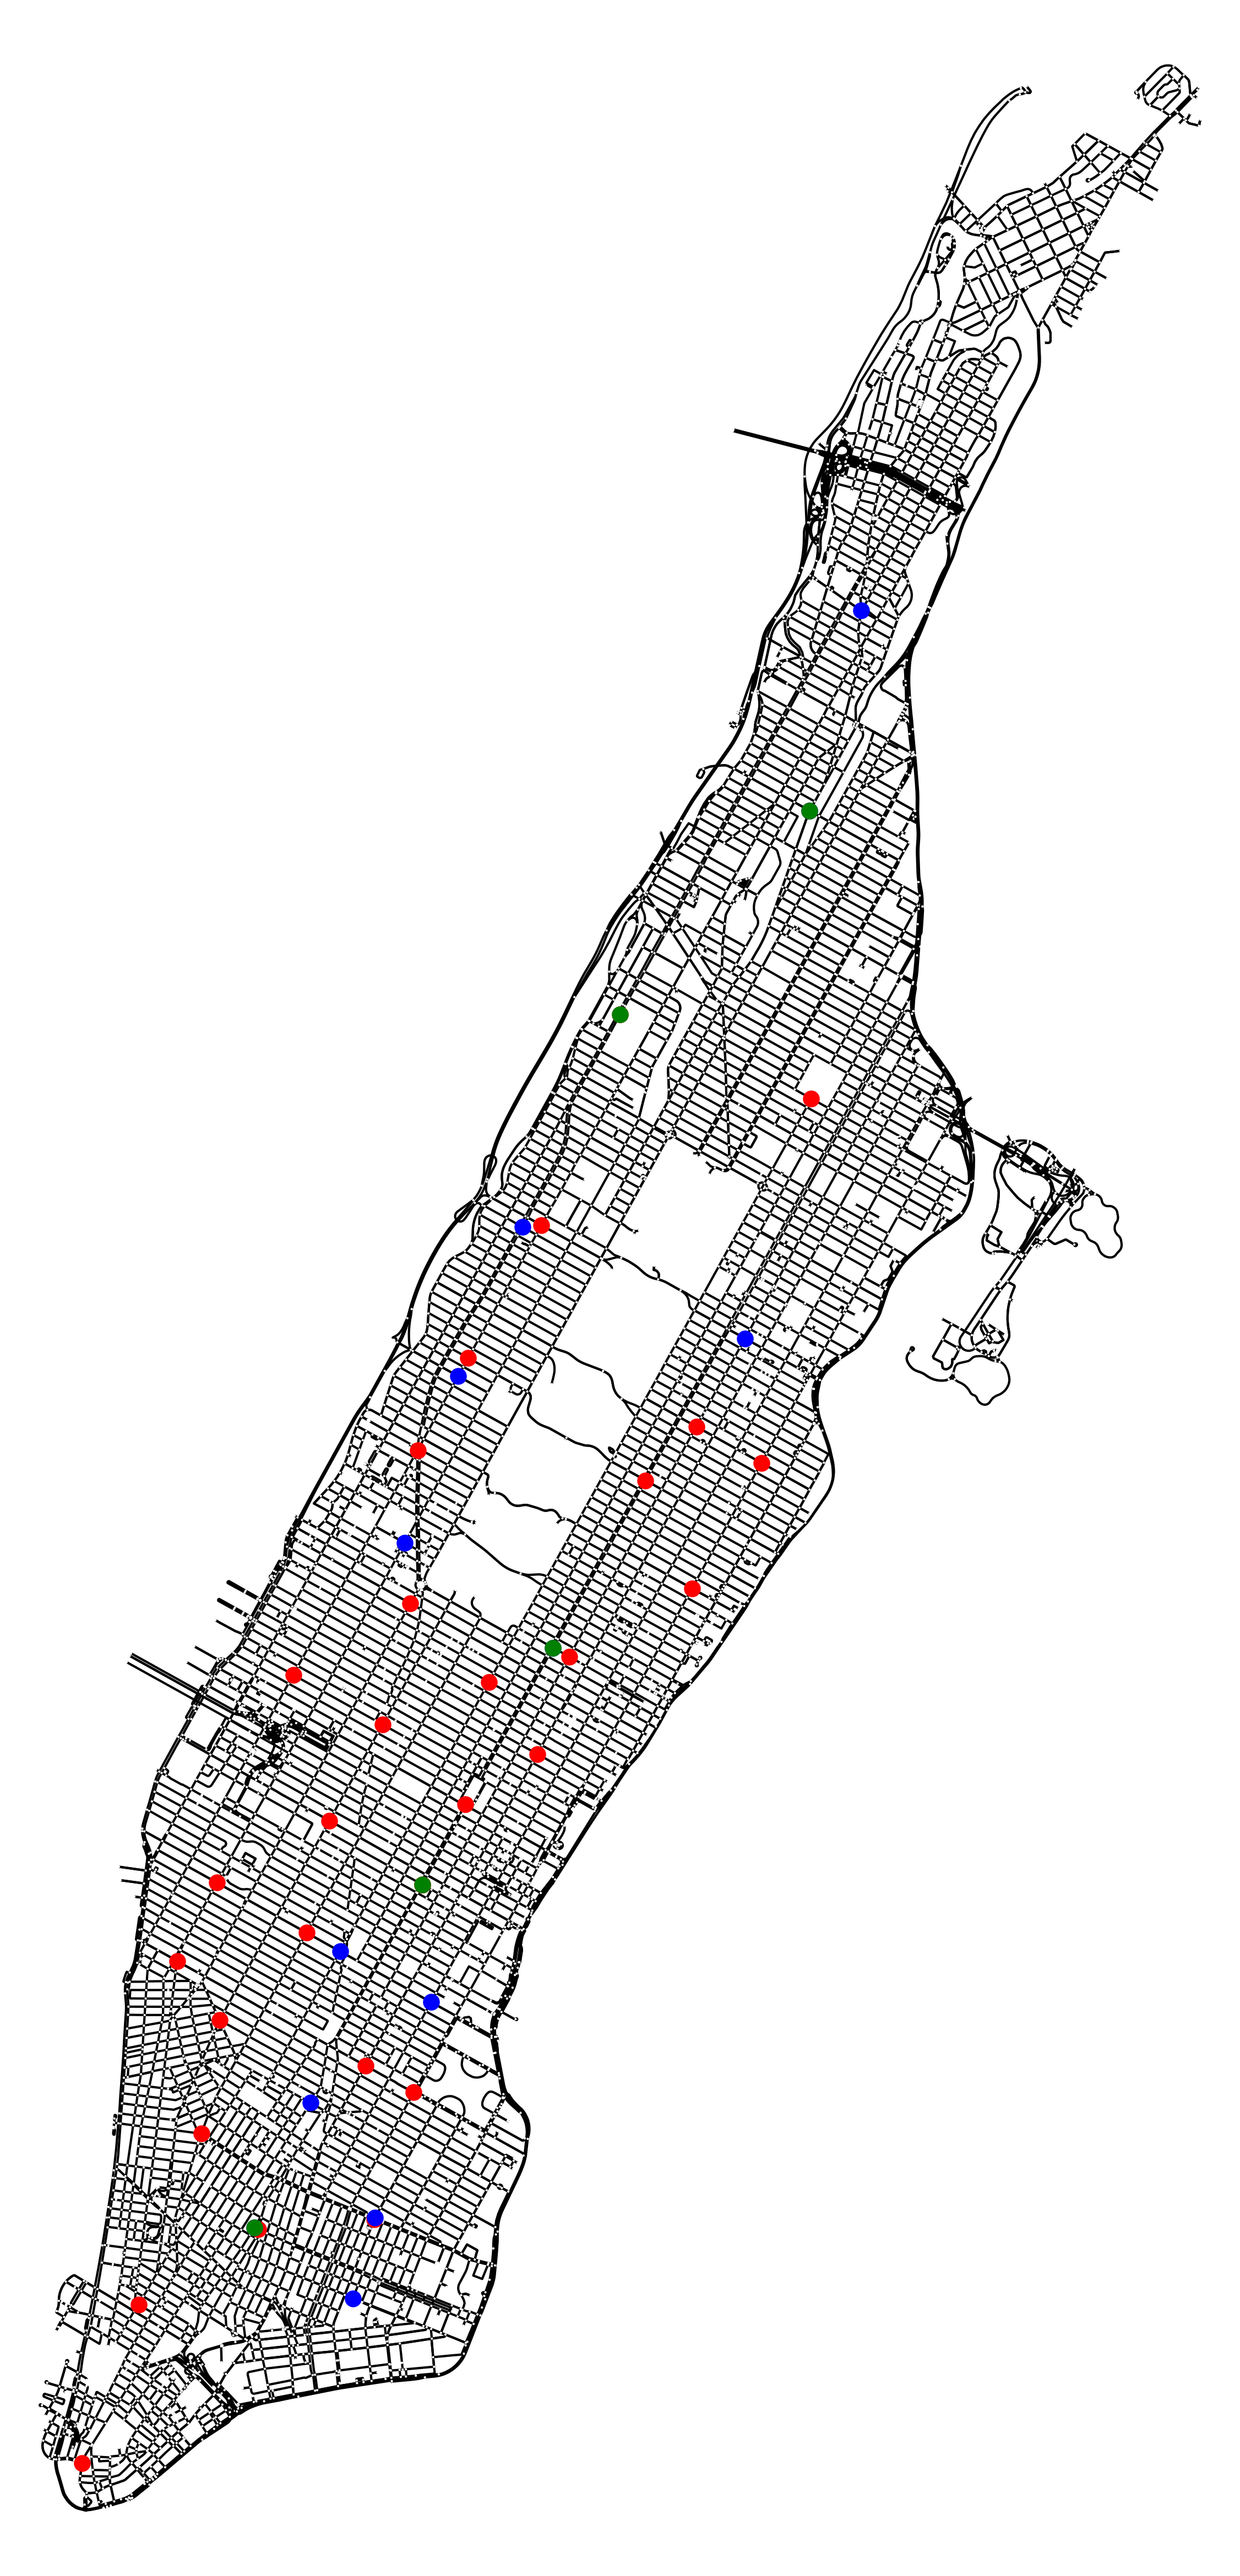
\includegraphics[width=\textwidth]{assets/img/07_graph_based/new_york_vanilla_info.png}
		\caption{}
		\label{fig:nyc_rn_info}
	\end{subfigure}
	\begin{subfigure}[b]{0.32\textwidth}
		\centering
		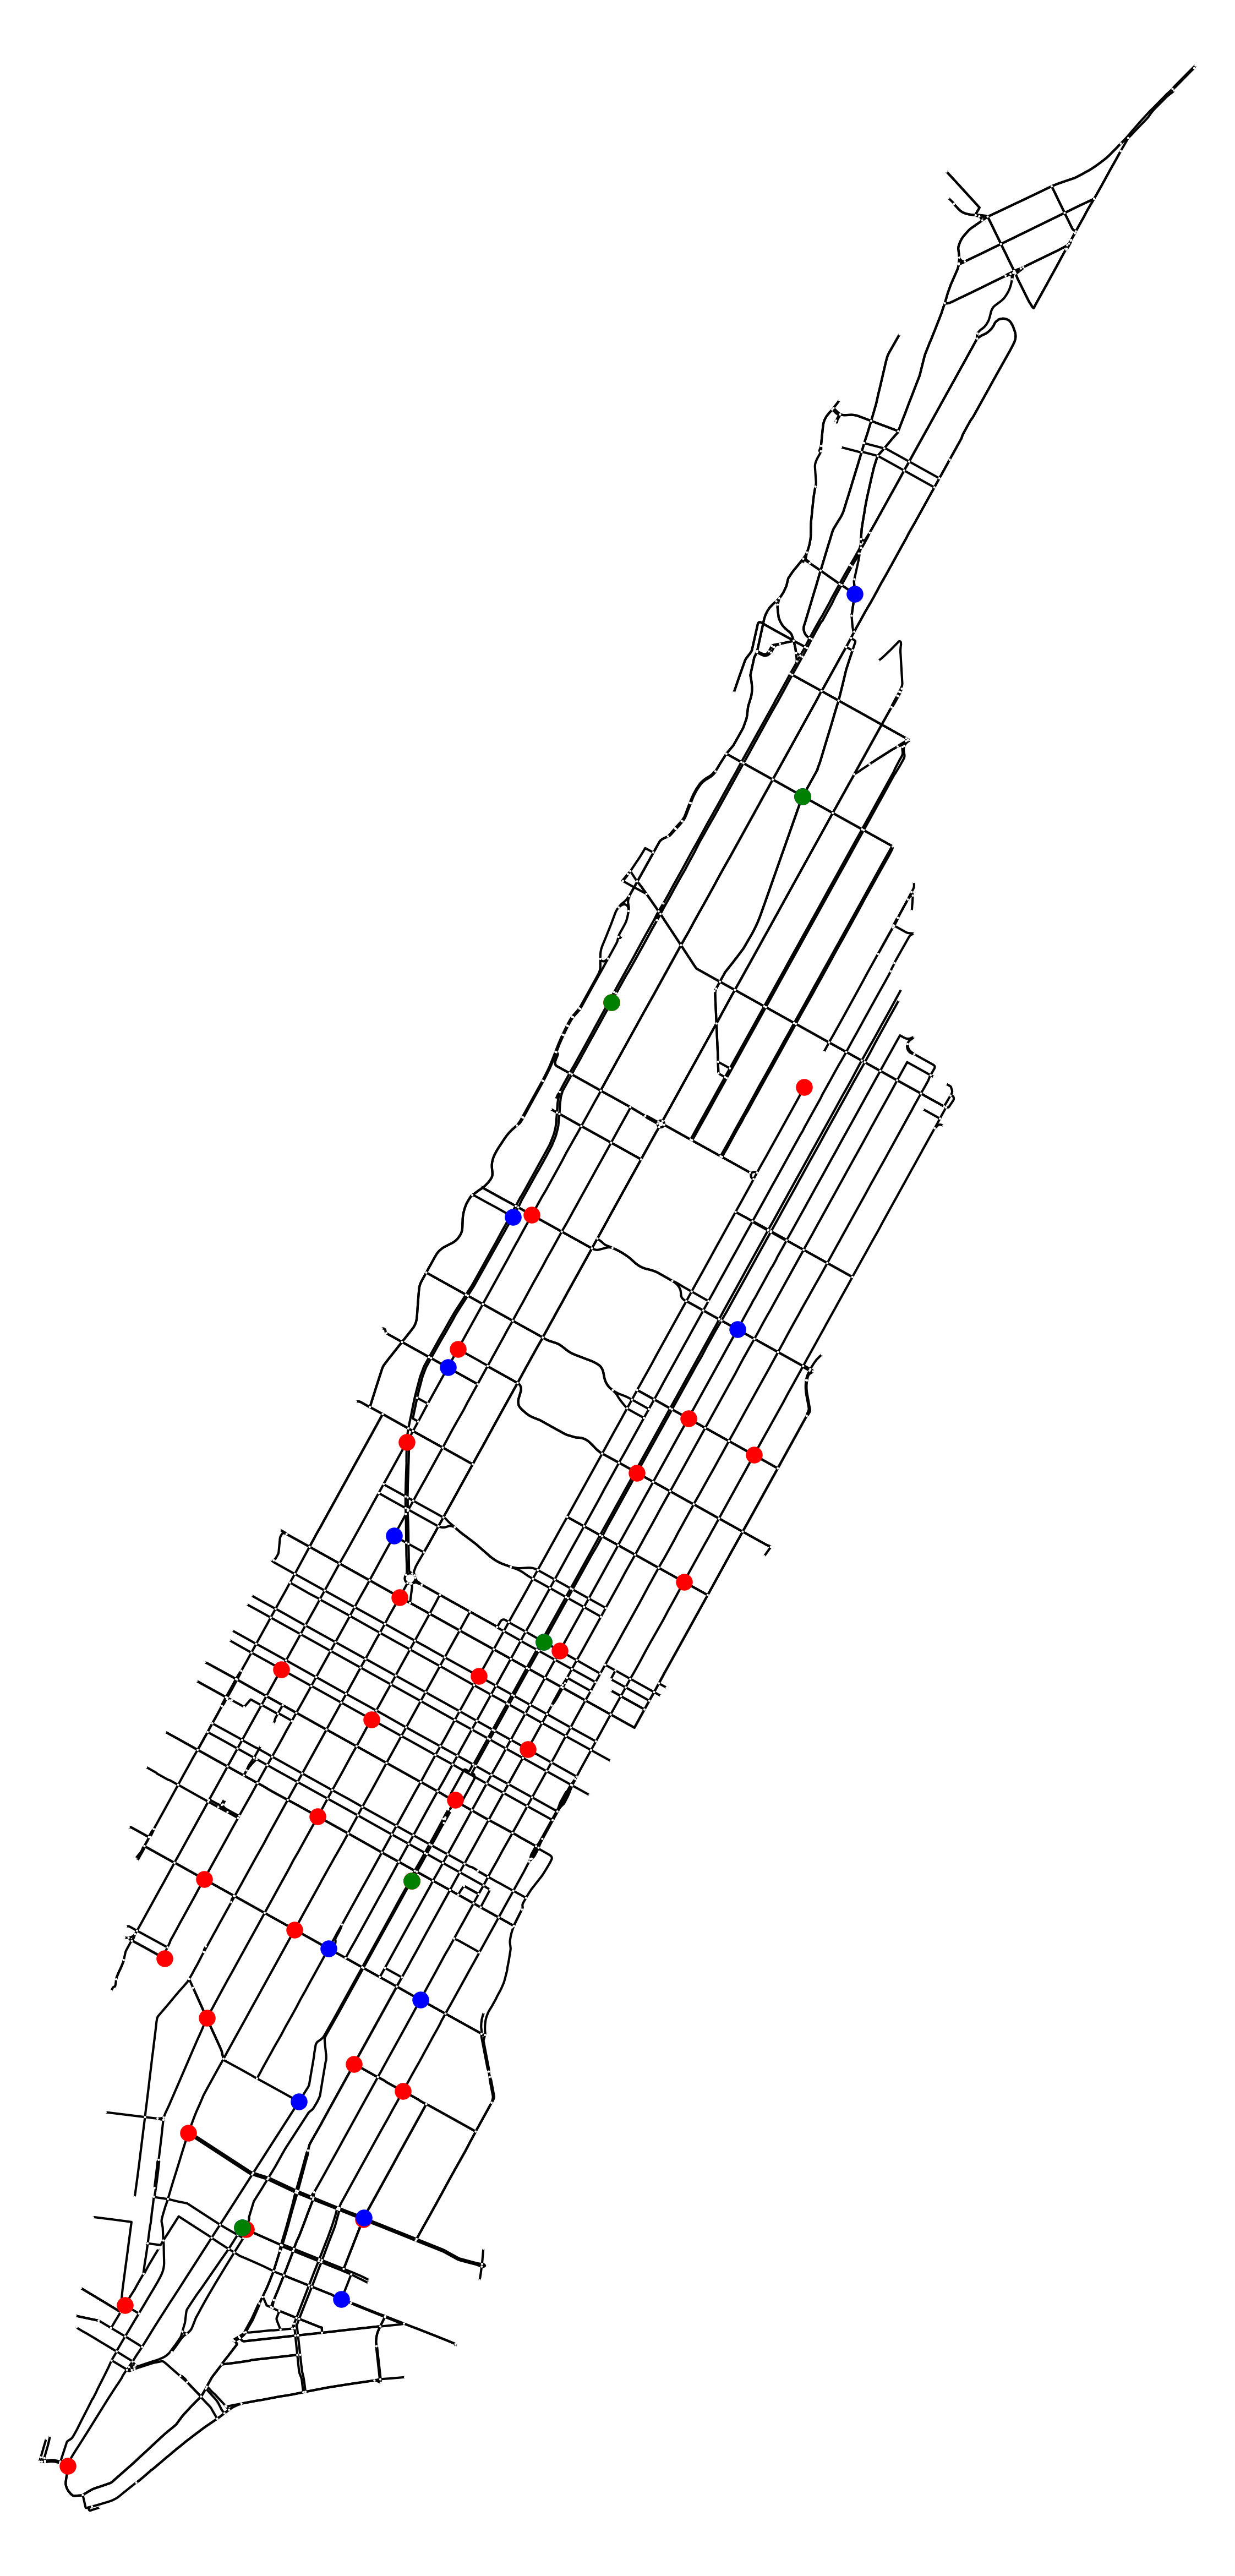
\includegraphics[width=\textwidth]{assets/img/07_graph_based/new_york_simplified_info.png}
		\caption{}
		\label{fig:nyc_simplified_info}
	\end{subfigure}
	\begin{subfigure}[b]{0.32\textwidth}
		\centering
		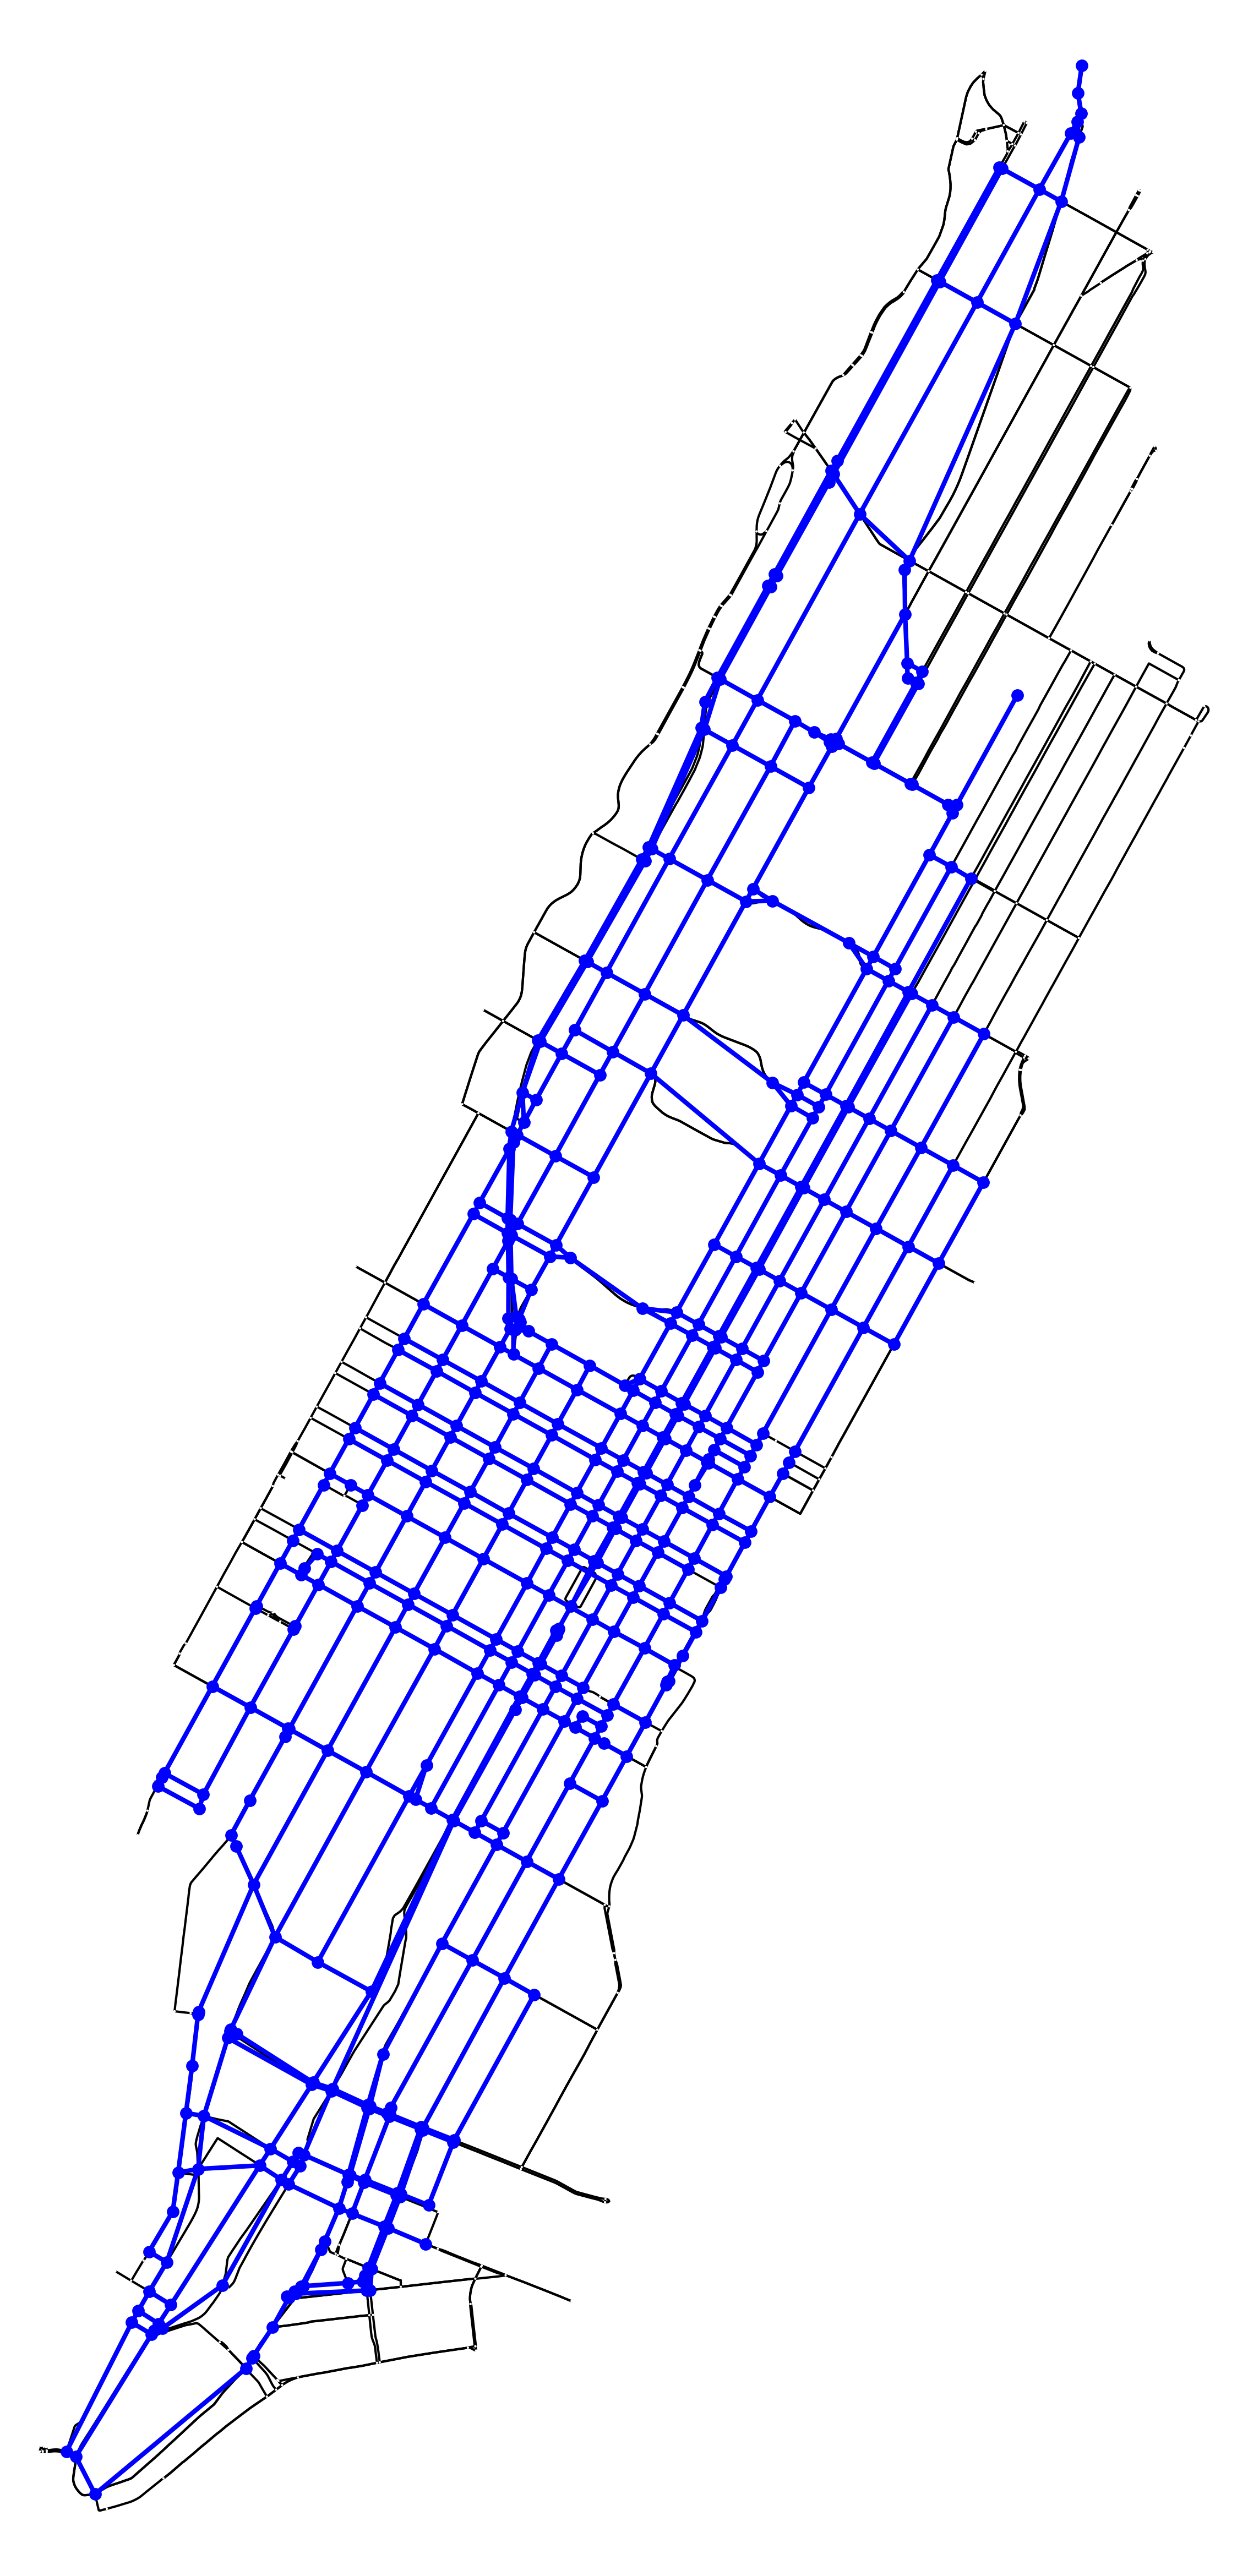
\includegraphics[width=\textwidth]{assets/img/07_graph_based/new_york_simplified_roads.png}
		\caption{}
		\label{fig:nyc_simplified_roads}
	\end{subfigure}
	
	\caption[Manhattan's Road Network Representation]{Manhattan's Road Network Representation. In \subfigref{fig:nyc_rn_info}, red points are used to indicate pick-up stations, while blue delineates drop-off points and green is used to pin-point the fictitious depots. These are obtained by the historical data. Furthermore, pick-up points can also be used as drop-off, and viceversa. \subfigref{fig:nyc_simplified_info} shows the semplified road network consisitnf of only the most important streets. Finally, \subfigref{fig:nyc_simplified_roads} shows the final version of the road network after the application of the minimum spanning tree algorithm.  }
	\label{fig:nyc_rn}
\end{figure}
The main purpose of this use case is to demonstrate the applicability of the model in the real world and the feasibility of the solutions presented in \secref{sec:ats_challenges_analysis} and \secref{sec:catsm}. This use case is based on real-world data extracted from taxi rides in manhattan in 2016 (\cite{Donovan2014}). \\
The data has been prepared in the following way. Since the data retrieved is based on the whole New York City, in order to decrease the complexity, some filters have been applied to only target the Manhattan area. More specifically, the pick-up and drop-off points which were outside of Manhattan have been filtered out. Subsequentially, these pick-up and drop-off points have been clustered in 40 locations. Finally, these locations have been mapped to the real Manhattan road network and the shortest path between five neighbours nodes has been traced in order to create a simplified road network, which can be seen in \figref{fig:nyc_rn}. The graph considered has 482 locations and 1622 routes. \\
As a consequence, the complexity of Manhattan's road network has been significantly reduced. Within the context of this project, and specifically in this section, this simplification is deemed acceptable since only proof of concepts are being considered. Furthermore, employing a more intricate representation of the road network would not significantly enhance the objectives at hand. This streamlined approach not only facilitates clearer demonstration of concepts but also expedites the analysis process, enabling a more focused examination of essential elements. Thus, for the current scope of this work, the simplified representation remains suitable and pragmatic.
According to the discussion in \secref{sec:rebal}, the region has been divided in multiple areas as well. This can be observed in \figref{fig:nyc_rn_info}. Although the division in areas it's not explicitely stated, five green-highlited nodes can be observed. These nodes represent depots and have been created to fulfill the same purpose of \secref{sec:rebal}.  In order to improve the performance of the simulation, the road network has been simplified by considering only the most important streets in Manhattan, as shown in \figref{fig:nyc_simplified_info} and \figref{fig:nyc_simplified_roads}. This approach optimizes resources while still providing valuable insights into the model performance. \figref{fig:nyc_simplified_roads} specifically has been obtained by first applying the Minimum Spanning Tree (MST) algorithm (\cite{networkx2021}) to the relevant nodes for the requests. The MST is used to calculate the smallest possible connected subtree that spans all the vertices in a given graph. In essence, constructing MST involves iteratively selecting edges with the smallest weight while ensuring that no cycles are formed. This process starts with any arbitrary vertex and gradually expands by adding the lightest edge connected to the existing tree until all vertices are encompassed. The connectiones between the nodes in the resulting MST graph have been restored using the original road network's street information to maintain the connectivity.\\
While information regarding passenger demands are relatively easy to obtain, other data must be crafted or estimated. In particular, details about the constraints outlined in \secref{sec:vc_model} can be challenging to gather as they are often specific to certain scenarios or dependent on external factors not captured by the model. For instance, determining the threshold in the congestion model is complex, especially considering it could easily reach thousands in a densely populated city like NYC. Likewise, the time windows of a request is also very specific to the application. For the rest of this work, this information will be derived from the available data and created, if required. For example, the traveling time for each link $T^a_{u,v}$ can be derived with the assumption of a constant speed. Trivially, since the distance is known, the travelling time can be calculated as follows: \\
\begin{equation}
	T^a_{u,v} = \dfrac{d_{u,v} }{l_{u,v}}
\end{equation}
where $l_{u,v}$ is the speed limit of the link $\langle u,v\rangle$. \\
Although data on customer mobility is readily accessible, obtaining precise information on goods delivery poses a challenge. This includes details on the specific category of goods being transported and the exact dropoff locations. Multiple might be the reasons for it, such as privacy, commercial sensitivity or due to the highly heterougenous nature of this field. Nevertheless, a potential approach to glean insights into goods delivery could involve leveraging publicly accessible datasets such as the GetFood Historical Data (\cite{getfoodnyc}). Amid the COVID-19 pandemic, initiatives like GetFoodNYC have been instrumental in facilitating emergency home food delivery for residents unable to access food through conventional means. Although the data provided does not contain delivery location, this can be simulated by picking a random location within the road network and the quantity can be estimated by the available data.\\
The simulations have been carried out using the CBC (\cite{schumacher2022rcbc}) and Gurabi (\cite{gurobi}) solvers used in combination with PuLP (\cite{dunning2011pulp})\footnote{On a 2018 Intel i7 MacbookPro}. 


\subsection{Rebalancing-Free ATS Analysis}
This use-case refers to the RDR (\algoref{RDR}) with the alternatives defined in (\ref{eq:flow_cons_arrival_graph_u_d2})-(\ref{eq:flow_cons_departure_graph_u_d2}) and the goal is to serve as many requests as possible, i.e. to minimize the cost function in \equaref{eq:req_served}.  For this use-case, since the rebalancing is not considered, the end depots are chosen randomly at the beginning of the simulation and only the starting and ending depots of transporting vehicles are exchanged at every iteration. As a result, transporting vehicles move from starting to end depot at one iteration and viceversa at the next iteration. Two main aspects are considered, namely charging time and congestion constraints. These two variables, which greatly influence the system's performance, have been varied to analyse how the system behave with \textit{(i)} high roads capacity low requests rate, i.e. high charging times, since vehicles can start moving after their battery has been charge with an additional 40\%; \textit{(ii)} same road capacity, but high request rate ( additional 5 \% of charging); \textit{(iii)} low road capacity and high charging rate; finally \textit{(iv)} lower capacity, but higher charging rate. 
 The details of the simulations are shown in \tabref{tab:routingless_simu_details} and the starting distribution of the vehicles in the depot is described in \tabref{tab:routingless_depot_distribution}. The overall performance is summarized in \tabref{tab:routingless_simu_performance}\footnote{Further information can be found in  \appref{appendix:additional_info}
 }.  \\




\begin{table}[h]
		\centering
		\begin{tabular}{ |l| c|c|c|c|c|}
			%\hline
			%	\multicolumn{2}{|c|}{Simulation Details} \\
			\hline
			&Sim. 1 & Sim. 2& Sim.3&Sim. 4&Sim. 5 \\
			\hline
			Vehicles \#& 24&-&- &-&-\\
			Iterations & 10&-&-&-&-\\
			Requests / $i$ & 10&-&-&-&-\\
			Charging \% / $i$ & 60&40&30&10&30\\
			$c_{u,v}$  / $i$ & 50&-&-&5&5\\
		\end{tabular}
		\caption[Details of the Rebalancing-less Simulation]{Details of the Rebalancing-less Simulation. ``$i$'' stands for iteration and ``-'' means the entry has not been changed from the previous one}
		\label{tab:routingless_simu_details}   
\end{table} 
	\begin{table}[h]
	\centering
	\begin{tabular}{ | p{2cm} | c | c | c | c |c|}
		\hline
		Depot ID & 1 & 2 & 3 & 4 & 5\\
		\hline
		\# Vehicles & 3 & 6 & 8 & 4 & 3\\
	\end{tabular}
	\caption{Depot Distribution Used During the Simulation}
	\label{tab:routingless_depot_distribution}   
\end{table}


\begin{table}[h]
	\centering
	\begin{tabular}{ |p{3.7cm}|c|c|c|c|c|}
		%\hline
		%\multicolumn{2}{|c|}{Depot Distribution} \\
		\hline
		& Sim. 1 & Sim. 2 & Sim. 3 & Sim. 4 & Sim. 5 \\
		\hline
		Total Distance (m)     &731993& 749006   & 824307 & 585955& 718618 \\
		Average Distance (m)  &30500 & 312089  & 34346 & 24415& 29942\\
		Total Time (s)         &14640& 14980  & 16486 & 11719& 14372\\
		Average Time (s)      & 610& 624   & 687 & 488& 599\\
		Unique Road Used 				&1171&1137&1244&1021& 1170\\
		Request Served  (\%)&64 & 63   & 68 & 57&60 \\
		%235488.79
		%\hline
	\end{tabular}
	
	\caption[Overview of the System's Performance for Routing-less Simulation.]{Overview of the System's Performance for Routing-less Simulation. The unique road used entry counts how many different roads have been used during the simulation. In other words, it measures the sum of routes that have been travelled by at least one vehicle. }
	\label{tab:routingless_simu_performance}   
\end{table}
\begin{figure}[th]
	\centering
	\begin{subfigure}[b]{0.35\textwidth}
		\centering
		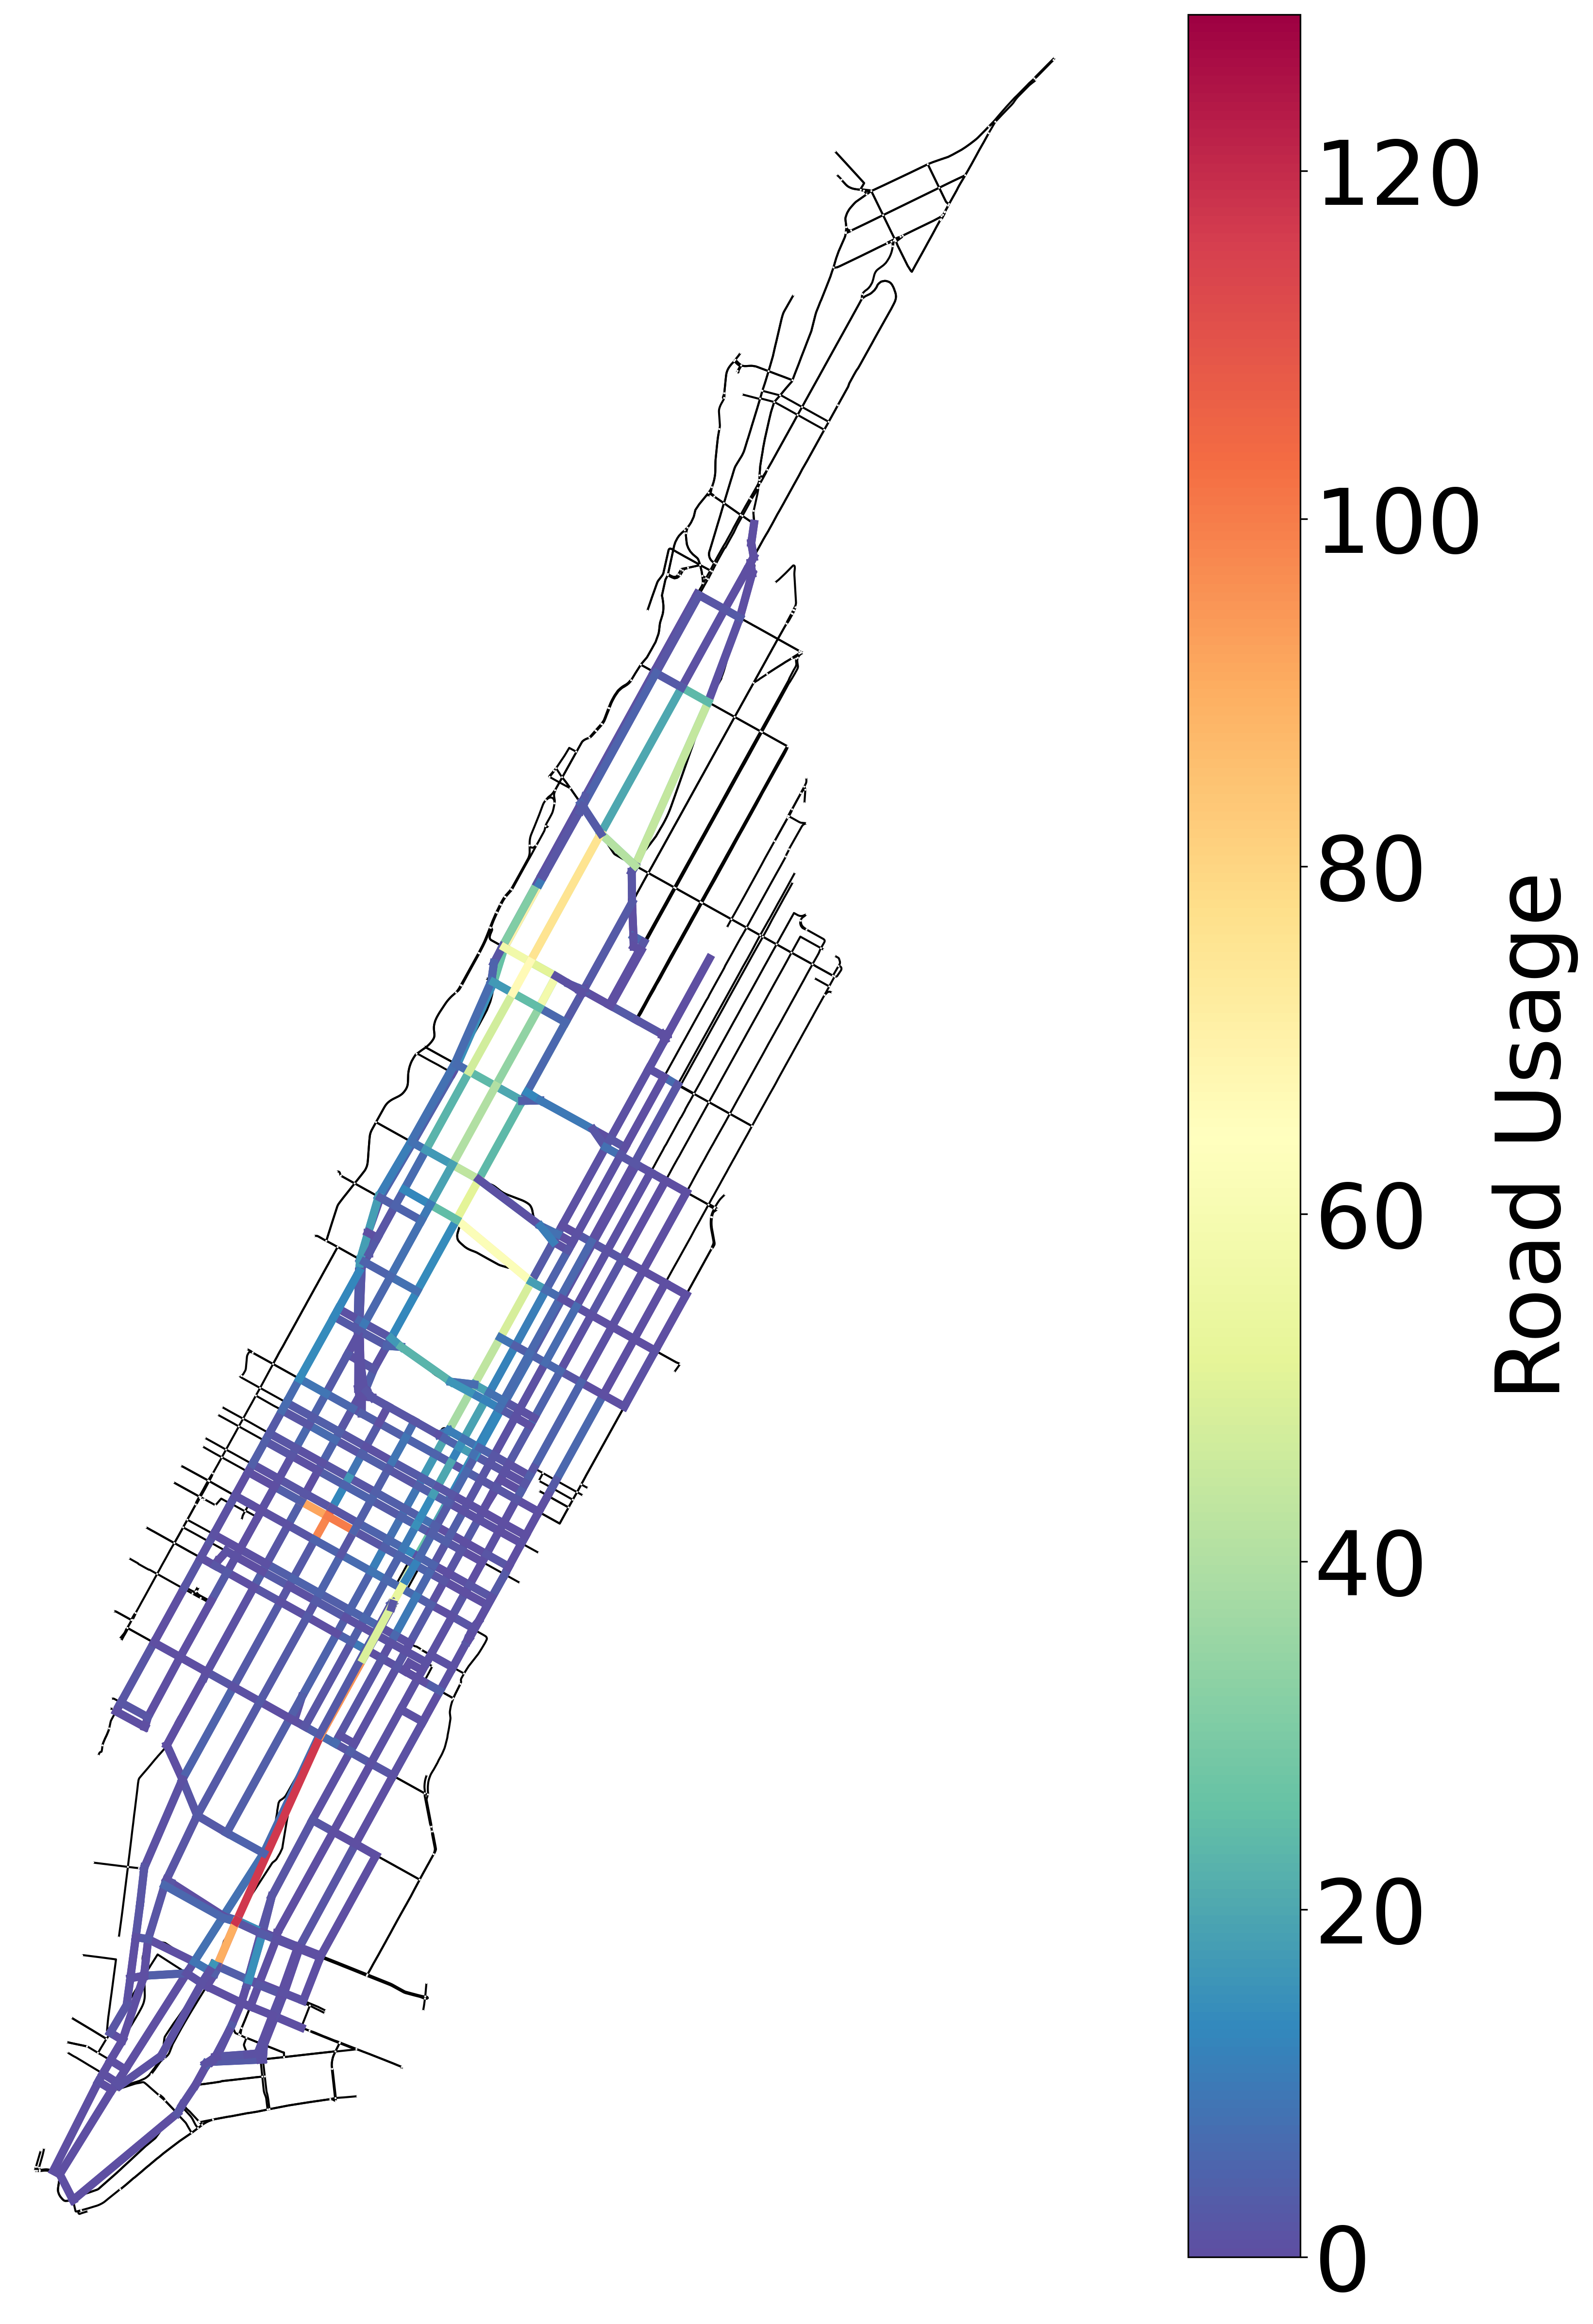
\includegraphics[width=\textwidth]{assets/img/07_graph_based/nyc_road_usage.png}
		\caption{}
		\label{fig:nyc_road_usage}
	\end{subfigure}
	\begin{subfigure}[b]{0.4\textwidth}
		\centering
		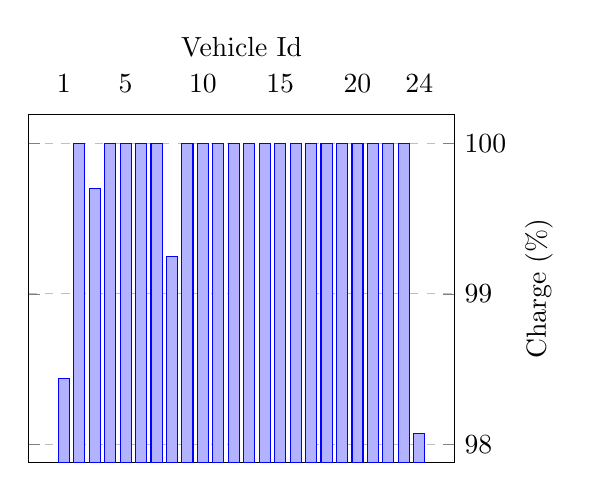
\begin{tikzpicture}
			\begin{axis}[
				ybar,
				xtick=data,
				xtick={1,5, 10,15,20,24},
				xlabel={Vehicle Id},
				ylabel={Charge (\%)},
				bar width=4pt,
				ymajorgrids=true,
				yticklabel pos=right,
				ylabel near ticks,
				grid style=dashed,
				xticklabel pos=right, xlabel near ticks,
				minor x tick num=9,
				xtick style={draw=none},
				width=7cm, 
				height=6cm
				]
				\addplot coordinates{
					(1,98.43523210637584)
					(2,100.0)
					(3,99.70028911971025)
					(4,100.0)
					(5,100.0)
					(6,100.0)
					(7,100.0)
					(8,99.25079230563661)
					(9,100.0)
					(10,100.0)
					(11,100.0)
					(12,100.0)
					(13,100.0)
					(14,100.0)
					(15,100.0)
					(16,100.0)
					(17,100.0)
					(18,100.0)
					(19,100.0)
					(20,100.0)
					(21,100.0)
					(22,100.0)
					(23,100.0)
					(24,98.07205105270594)
				};			
			\end{axis}
		\end{tikzpicture}
		\caption{ }
		\label{fig:charge_vehicle_baseline}
	\end{subfigure}
	\caption[Overview of System's Performance without Congestions]{ 
		\subfigref{fig:nyc_road_usage} illustrates the utilization of the entire road network. Road usage is determined by aggregating the total number of vehicles traversing each road segment throughout the shift duration. The most used roads are shown in red, while blue indicates low activity.   \subfigref{fig:charge_vehicle_baseline} displays the average vehicle charge during the shifts.
	}
	\label{fig:nyc_analysis_no_congestions}
\end{figure}







In a system characterized by wide charging times and absence of congestion limits ($c_{u,v} > |\mathcal{A}| \quad \forall (u,v) \in \mathcal{E}$), the performance depicted in \figref{fig:nyc_analysis_no_congestions} unfolds. Notably, the objective is not focused on minimizing overall travel time \equaref{eq:travel_time_routing} or total distance traveled \equaref{eq:distance_time_routing}, but rather on maximizing the number of served requests. Consequently, with more charging time and less road constraint, vehicles tend to cover more distance. This inclination is further facilitated by the lack of real capacity constraints on roads and the freedom for vehicles to traverse them at any time.\\
As a consequence, the utilization of the road network is uneven, as illustrated in \figref{fig:nyc_road_usage}, where the most-utilized links are highlighted in red. This uneven distribution can be attributed partly to the concentration of drop-off and pick-up points, as well as depots, primarily within downtown Manhattan. However, the presence of a depot uptown causes an area of relatively high vehicles activity, although there are not many relevant location there, as shown in \figref{fig:nyc_simplified_info}. This suggests that if the aim is to mitigate vehicle usage and road congestion, this region shouldn't exhibit high vehicular activity. This consideration becomes significant when addressing rebalancing strategies.  \\
Furthermore, \figref{fig:charge_vehicle_baseline} suggests that most of the vehicles have not been used during the shift. This can be inferred by observing that, for half of the vehicles, the average charge is exactly 100\%, i.e. the same as the starting battery charge. This suggests that the fleet of vehicles could  be reduced in number and maintaining the same capacity. \\
\figref{fig:nyc_analysis_charging} shows the same metrics for the third simulation. Although the charging time is reduced in half, this simulation results in a much more efficient use of the road network. First of all, as shown in \tabref{tab:routingless_simu_performance}, more requests could be served in the same amount of time. Furthermore, although with less charge, vehicles tend to travel more. Though it may seem counterintuitive, the reason could be that the solver has been limited to ten minutes. As a result of this restriction, it is likely that, within this time limit, the solver has been able to prune out unfeasible solutions thanks to the more stringent requirement. Furthermore, from \figref{fig:nyc_road_usage_charge}, contrary to \figref{fig:nyc_road_usage}, it is evident that the road network is used more evenly. As expected, there are still roads that stand out as the most used ones, which reflects the result obtained previously and it is still to associate with the fact that terminal depots are not assigned properly. 
 On the contrary, as shown in \figref{fig:charge_vehicle_limit_charge}, the fleet usage is similar when compared to previous approaches. Although the distribution of average charge appears to be slightly more uneven compared to \figref{fig:charge_vehicle_baseline} , with some vehicles maintaining an average charge of around 90\%, most vehicles are not used entirely. This suggests that the fleet could be reduced in this case as well. Although vehicles do not fully recharge at the end of each shift, according to their evolution over the simulation period \footnote{The evolution of a set of vehicles can be found in \figref{fig:ex_soc_vehicles}}, since the fleet is generously big, other vehicles can replace charging vehicles for the shift. On the one hand, this results on more vehicles used, however the overall average is well above 80\% at the end of the shift.  

\begin{figure}[th]
	\centering
	\begin{subfigure}[b]{0.35\textwidth}
		\centering
		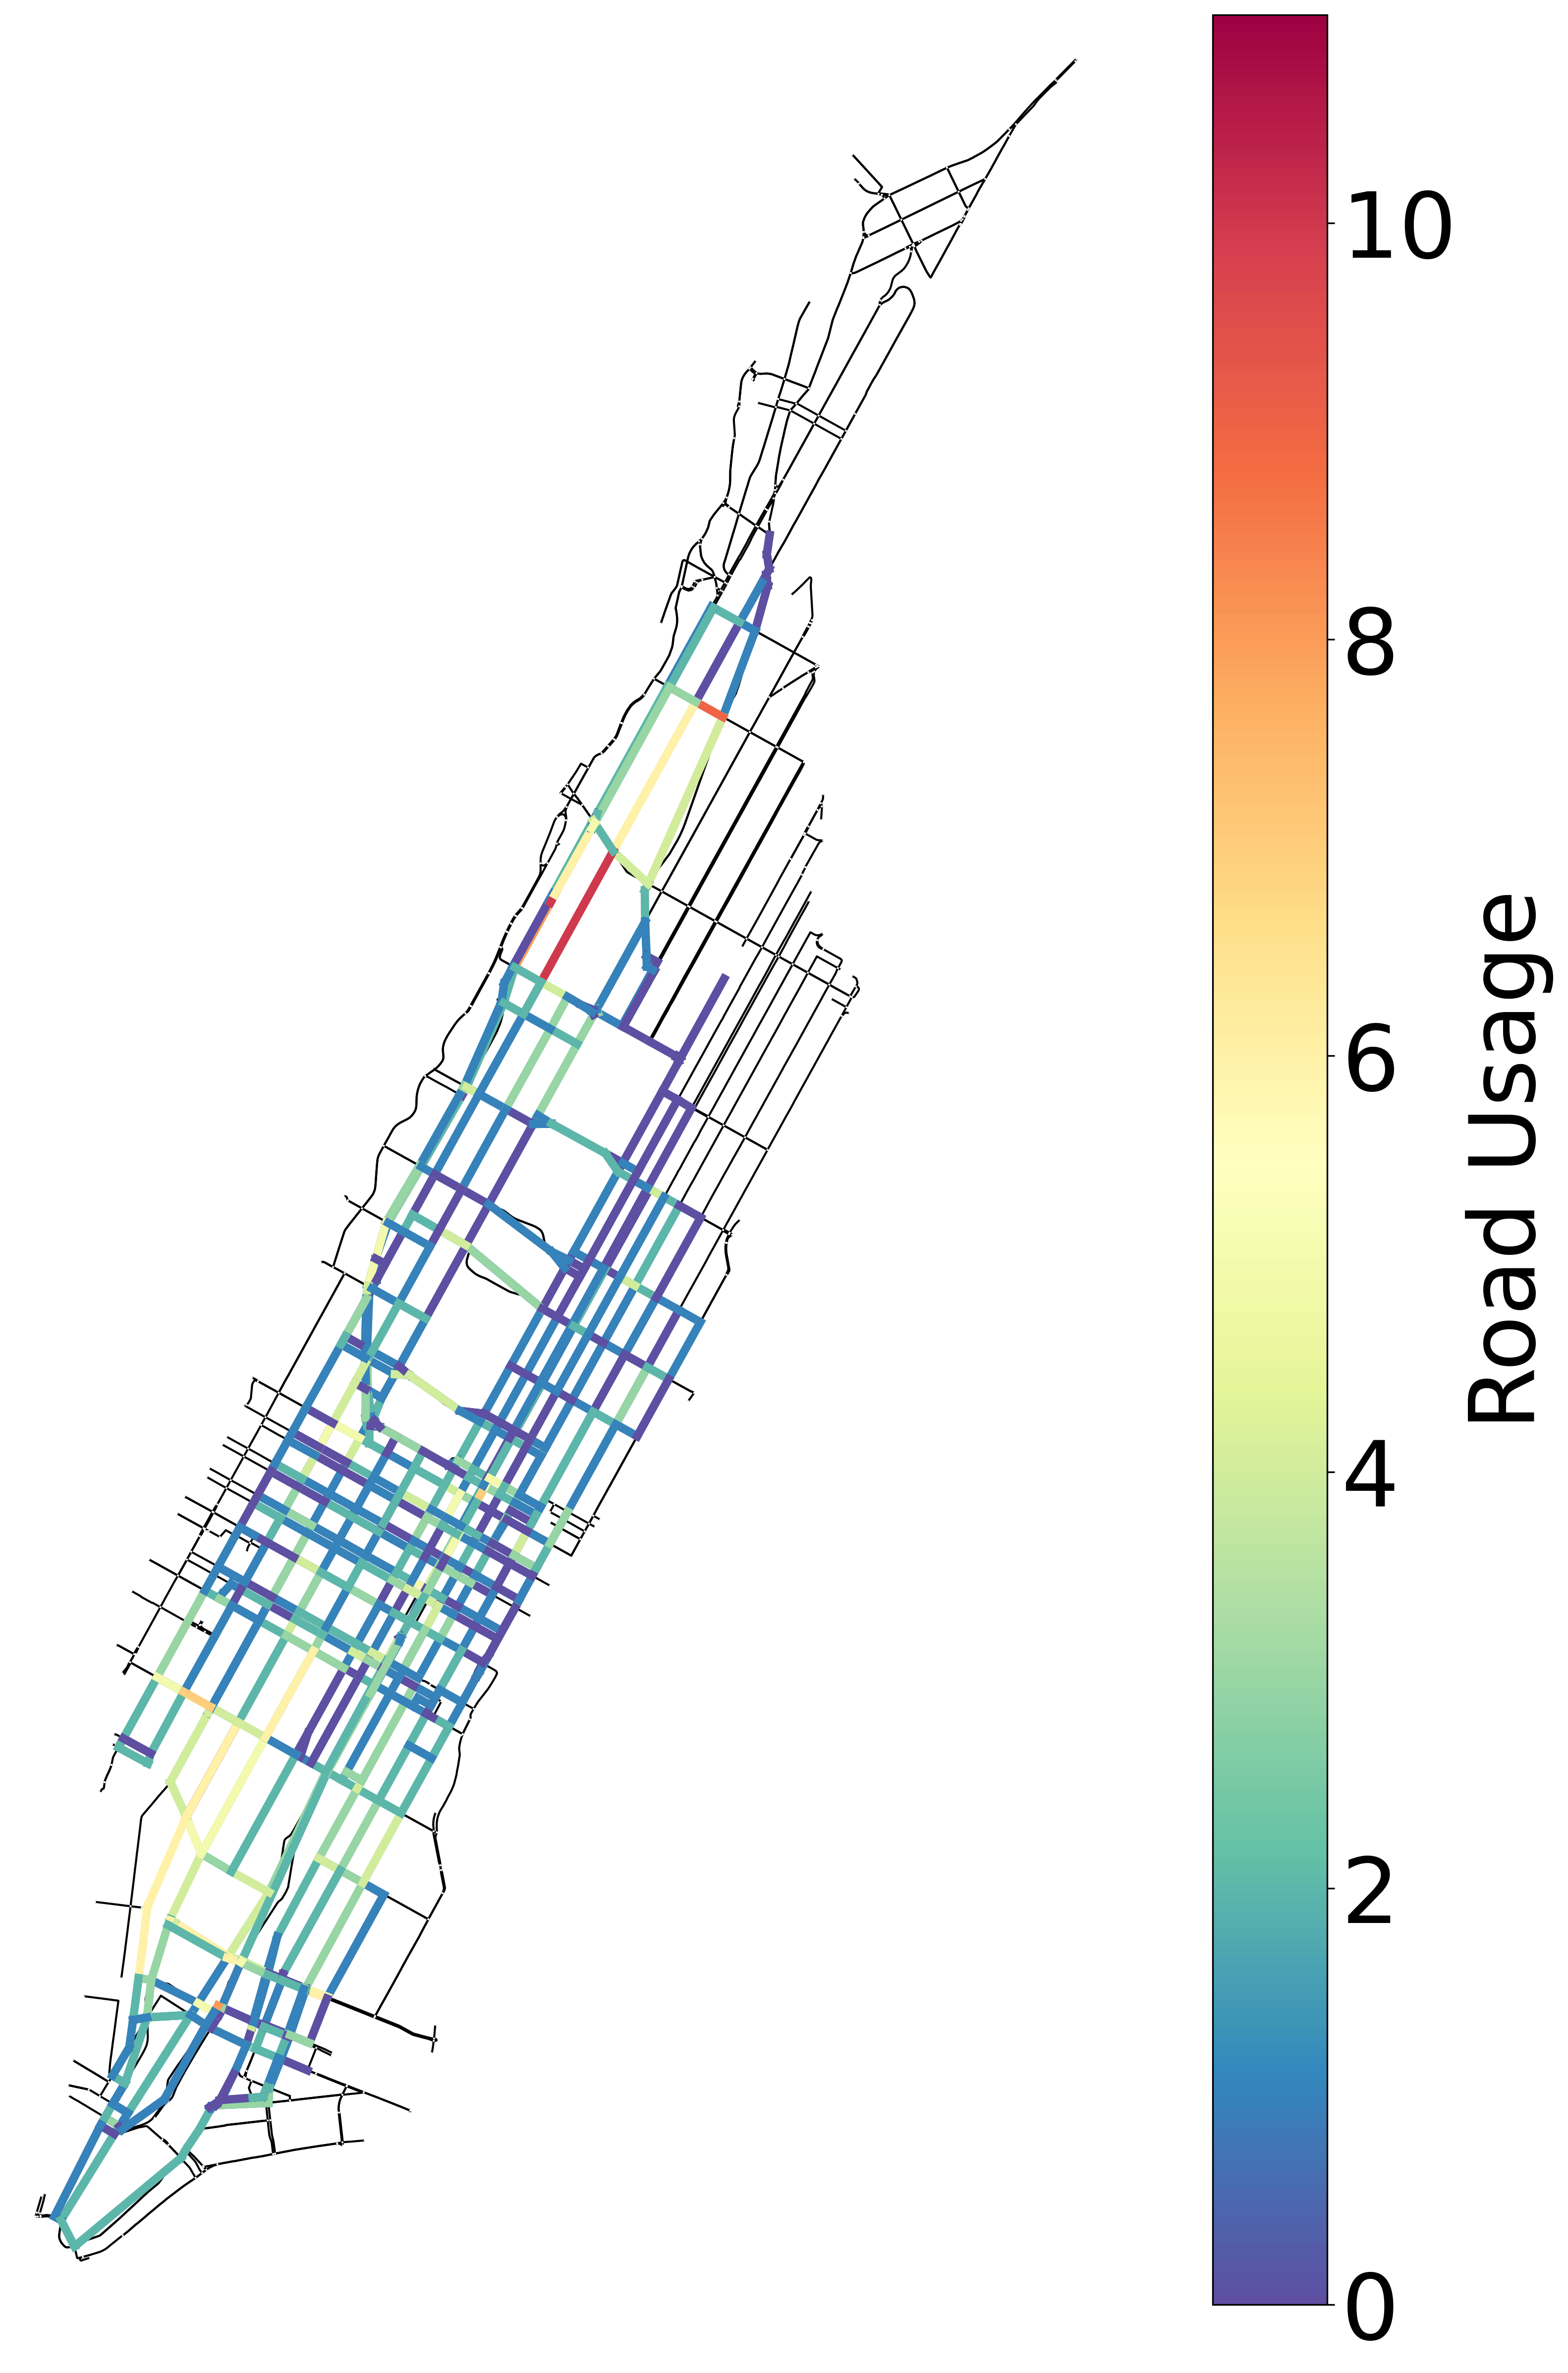
\includegraphics[width=\textwidth]{assets/img/07_graph_based/nyc_road_usage_charging.png}
		\caption{}
		\label{fig:nyc_road_usage_charge}
	\end{subfigure}
	\begin{subfigure}[b]{0.4\textwidth}
		\centering
		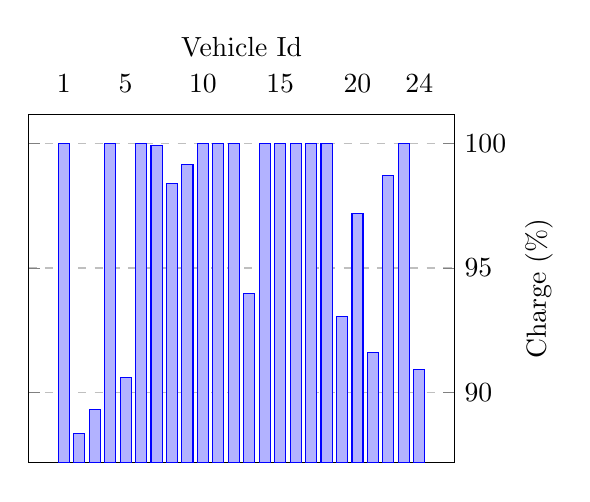
\begin{tikzpicture}
			\begin{axis}[
				ybar,
				xtick=data,
				xtick={1,5, 10,15,20,24},
				xlabel={Vehicle Id},
				ylabel={Charge (\%)},
				bar width=4pt,
				ymajorgrids=true,
				yticklabel pos=right,
				ylabel near ticks,
				grid style=dashed,
				xticklabel pos=right, xlabel near ticks,
				minor x tick num=9,
				xtick style={draw=none},
				width=7cm, 
				height=6cm
				]
				\addplot coordinates{
					(1,100.0)
					(2,88.35905320863947)
					(3,89.33530101077898)
					(4,100.0)
					(5,90.61846304806419)
					(6,100.0)
					(7,99.91893531345714)
					(8,98.39234898425467)
					(9,99.1714923967497)
					(10,99.99845901113507)
					(11,100.0)
					(12,100.0)
					(13,93.98336252725261)
					(14,100.0)
					(15,100.0)
					(16,100.0)
					(17,100.0)
					(18,100.0)
					(19,93.05064515550362)
					(20,97.20717736304084)
					(21,91.61194803870156)
					(22,98.70594024174596)
					(23,100.0)
					(24,90.94137883728938)
				};			
			\end{axis}
		\end{tikzpicture}
		\caption{ }
		\label{fig:charge_vehicle_limit_charge}
	\end{subfigure}
	\caption{Overview of System's Performance for Routing-less Simulation 3.}
	\label{fig:nyc_analysis_charging}
\end{figure}


\begin{figure}[th]
	\centering
	\begin{subfigure}[b]{0.35\textwidth}
		\centering
		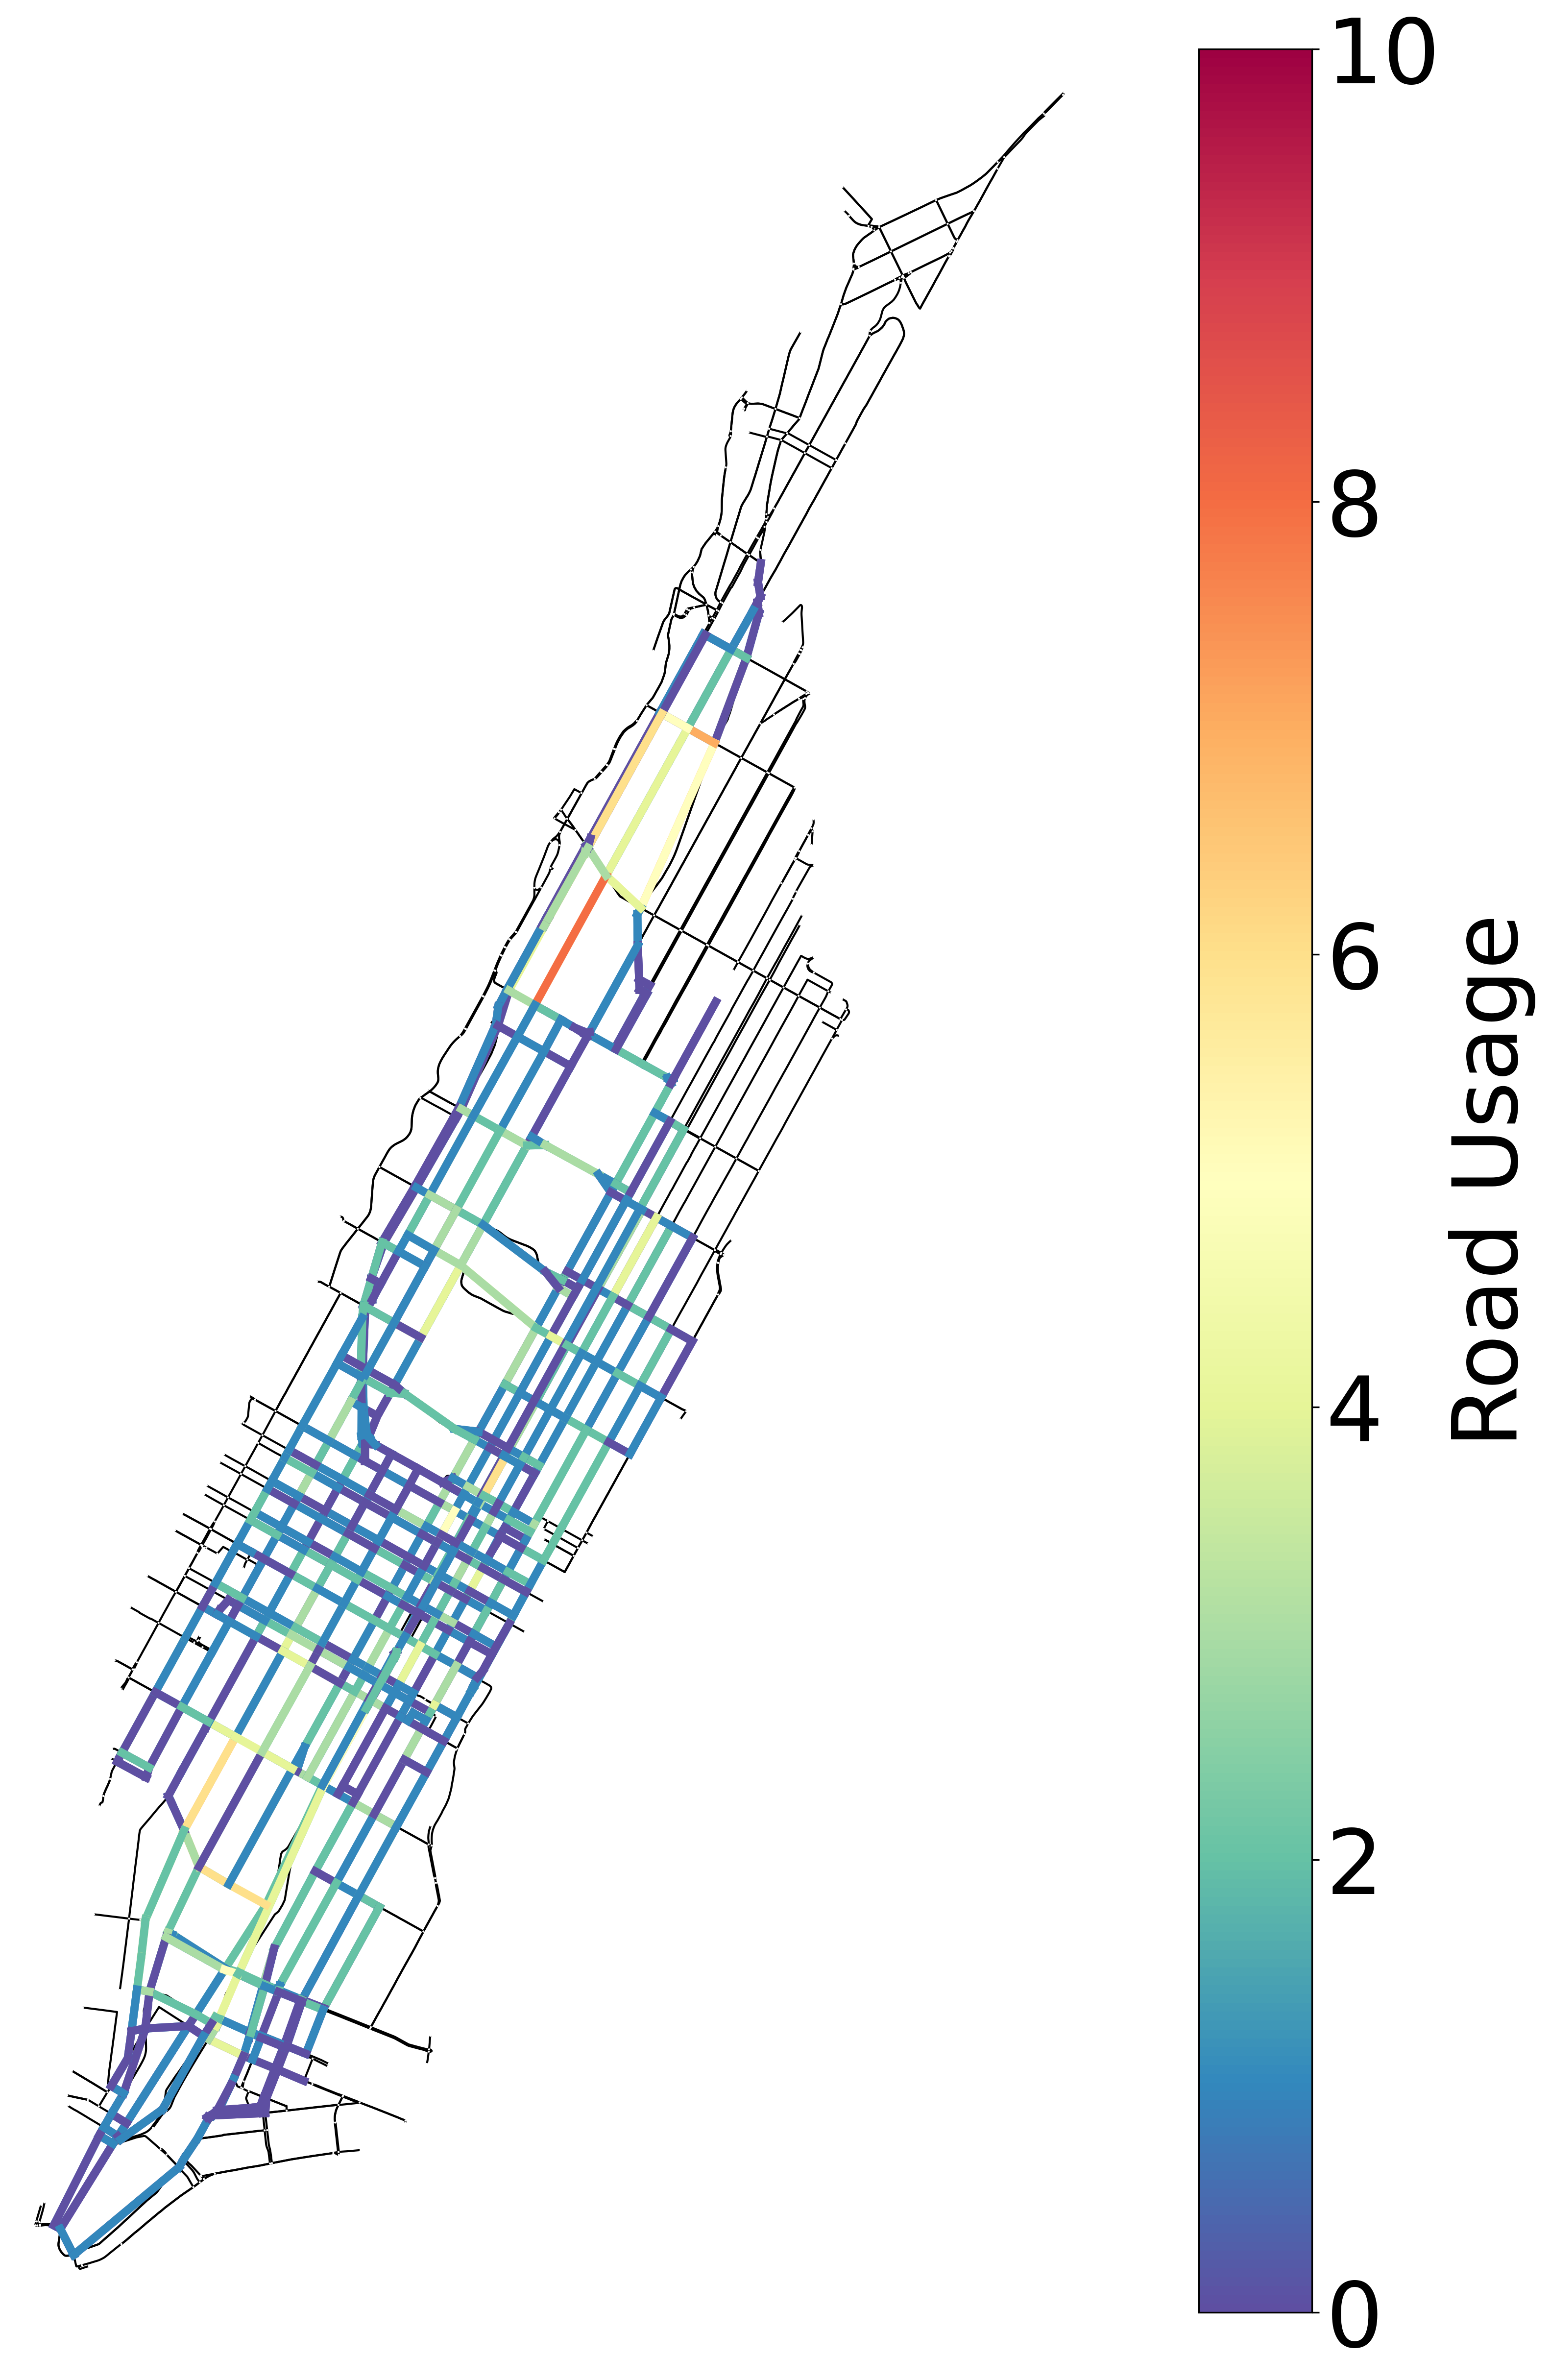
\includegraphics[width=\textwidth]{assets/img/07_graph_based/nyc_road_usage_cong.png}
		\caption{}
		\label{fig:nyc_road_usage_charg}
	\end{subfigure}
	\begin{subfigure}[b]{0.4\textwidth}
		\centering
		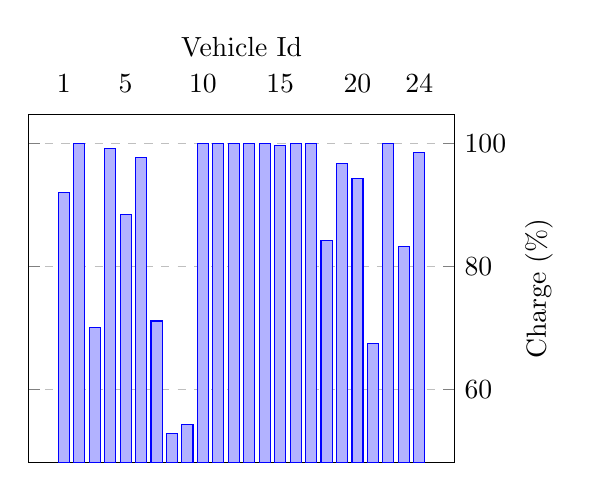
\begin{tikzpicture}
			\begin{axis}[
				ybar,
				xtick=data,
				xtick={1,5, 10,15,20,24},
				xlabel={Vehicle Id},
				ylabel={Charge (\%)},
				bar width=4pt,
				ymajorgrids=true,
				yticklabel pos=right,
				ylabel near ticks,
				grid style=dashed,
				xticklabel pos=right, xlabel near ticks,
				minor x tick num=9,
				xtick style={draw=none},
				width=7cm, 
				height=6cm
				]
				\addplot coordinates{
					(1,91.96815064537292)
					(2,100.0)
					(3,70.0641947932822)
					(4,99.1575051816054)
					(5,88.4183678168051)
					(6,97.72895458312098)
					(7,71.15084119314325)
					(8,52.86143074379152)
					(9,54.25630387855951)
					(10,100.0)
					(11,100.0)
					(12,100.0)
					(13,100.0)
					(14,100.0)
					(15,99.72301488888888)
					(16,100.0)
					(17,100.0)
					(18,84.20912254717499)
					(19,96.73937986838705)
					(20,94.287382511374)
					(21,67.55157749565974)
					(22,100.0)
					(23,83.31979792658574)
					(24,98.49139253136917)
				};			
			\end{axis}
		\end{tikzpicture}
		\caption{ }
		\label{fig:charge_vehicle_baseline_cong}
	\end{subfigure}
	\caption{Overview of System's Performance for Routing-less Simulation 4.}
	\label{fig:nyc_analysis_congestions}
\end{figure}
The performance of simulation number four can be observed in \figref{fig:nyc_analysis_congestions}. In this case, a more stringent approach for the congestion limit has been considered, i.e. no more than five vehicles can traverse a link at the same time. Furthermore, vehicles have only been charged up to ten per cent after each iteration. As a result, the fleet has been able only to serve up to 57\%. While the ten minutes limit on the solver is contributing, the strict capacity on the streets in combination with the low charging rate is resulting in a major downgrade in performance. The vehicles tend to travel less, for less time and can not reach all the requests. Since the graph is an abstraction of the real street network in Manhattan, one way roads are also modelled, therefore, reaching a particular node, might be hindered by a common link not being accessible by more than four vehicles at the same time. Furthermore, road capacity and charging limits have also a high influence on the fleet usage. As shown in \figref{fig:charge_vehicle_baseline_cong}, more vehicles tend to be used, as the overall charge is lower, with an average charge as low as below 60\% . The evolution of the vehicles with the lowest average charge over time shown in \figref{fig:ex_soc_vehicles2} suggests two main phenomena:  \textit{i} vehicles tend to be used for up to 50\% of the shift duration or until their charge is enough to cover the requests and \textit{(ii)} as soon as their charge is not enough to cover a batch of requests, they are not considered for a relatively long period of time. These two phenomena are clearly fleet dependend, since more vehicles in the fleet will accentuate them more and a lower one would imply a bigger need for every vehicle to be active. \\
A similar effect can be found by analysing simulation number five\footnote{The same metrics can be found in \figref{app:fig:nyc_analysis_congestions_simu5}
and \figref{fig:ex_soc_vehicles_simu5}}





\subsection{Rebalancing-Integrated System Analysis}
To ensure a comprehensive and and equitable comparison of vehicle rebalancing within the simulations, majority of the parameters have been kept consistent. \tabref{tab:rebalancing_with_simu} provides a summary of the primary parameters utilized in this simulation. The introduction of the rebalancing strategy, as outlined in \secref{sec:rebal}, was motivated by the primary objective of enhancing service fulfillment rates. By strategically redistributing vehicles across the transportation network, the aim was to ensure a more consistent and reliable service delivery to customers. However, this strategic move was not without its anticipated drawbacks, notably in the form of an expected increase in travel statistics, especially since the length of the route is not included in the system's objective. Therefore, the system's objective is a trade-off between the number of requests served and the number of rebalancing vehicles in order to decrease unnecessary travels. \\
\begin{table}[h]
	\centering
	\begin{tabular}{ |l| c|c|c|c|}
		%\hline
		%	\multicolumn{2}{|c|}{Simulation Details} \\
		\hline
		&Sim. 1 & Sim. 2& Sim.3&Sim. 4\\
		\hline
		%Vehicles \#& 24&-&- &-\\
		%Iterations & 10&-&-&-\\
		%Requests / $i$ & 10&-&-&-\\
		Charging \% / $i$ & 60&30&10&30\\
		$c_{u,v}$  / $i$ & 50&10&5&5\\
	\end{tabular}
	\caption[Details of the Simulation with Vehicle Rebalancing]{Details of the Simulation with Vehicle Rebalancing. Vehicles' number, iterations and requests for iterations have not been changed. Furthermore, the same requests have been picked for a more fair comparison.}
	\label{tab:rebalancing_with_simu}   
\end{table} 

\begin{table}[h]
	\centering
	\begin{tabular}{ |p{3.7cm}|c|c|c|c|}
		%\hline
		%\multicolumn{2}{|c|}{Depot Distribution} \\
		\hline
		& Sim. 1 & Sim. 2 & Sim. 3 & Sim. 4   \\
		\hline
		Total Distance (m)     &806280&   874937 & 871167 &  972776 \\
		Average Distance (m)  &33595 & 36456  &36299  & 40532 \\
		Total Time (s)         &16126&17499   &  17423& 19456 \\
		Average Time (s)      & 672&  729  & 726 &  811\\
		Unique Road Used 				&1193&1206&1186&1278 \\
		Request Served  (\%)&81 &  78 &  81& 79 \\
		%235488.79
		%\hline
	\end{tabular}
	
	\caption{Performance of the Simulation with Vehicle Rebalancing }
	\label{tab:rebalancing_simulation}   
\end{table}
The hypothesis has been confirmed by the simulation. \tabref{tab:rebalancing_simulation} contains a summary of the performance of this simulation. When comparing simulations with similar parameters, the impact of rebalancing on travel statistics becomes evident, with notable increases observed across all factors. Conversely, the number of served requests has notably risen across all simulations. Specifically, performance among simulations incorporating rebalancing remained relatively consistent, hovering around 80\%. This highlights the effectiveness of the rebalancing strategy in enhancing service fulfillment rates despite the associated increase in travel metrics. An additional goal associated with rebalancing was a more efficient vehicle use road network usage. \figref{fig:ex_soc_rebalancing_simu_2_3} shows the results measure for Simulation 2 and 3. Starting from \figref{fig:nyc_road_usage_rebalancing_simu_2} and \figref{fig:nyc_road_usage_rebalancing_simu_3}, when comparing it to previous results, the road usage did not improve. On the contrary, since vehicles are travelling to different depots potentially at every iteration, different routes must be taken. Interestingly, when observing the number of unique road used, this does not increase dramatically from the routing-less simulation. Furthermore, the road network analysis indicates a similar imbalance, where downtown and uptwon manhattan have the highest usage. Furthemore, the similar roads in both simulation measured a high usage. While this is against the previous hypothesis, i.e. that rebalancing would have decrease the usage uptown due to a lower amount of nodes, it offers another important hinsight. By observing the road usage in both cases, one is able to determine the most important streets and, therefore, able to make more informed decisions on how to manage the road network in the future. \\
\figref{fig:ex_soc_vehicles_rebalancing_simu_2} and \figref{fig:ex_soc_vehicles_rebalancing_simu_3} show the evolution of the state of charge for a set of vehicles. Compared to previous results, as expected, the charge of the vehicles is less consistent during the shift. During the process of rebalancing, vehicles often travel to various depots, resulting in fluctuating distances traveled. Consequently, this can lead to variations in the final charge of the vehicles, either lower or higher. While vehicles have been picked to show this fact, it is still worth noting that, as could be observed in \figref{fig:ex_soc_vehicles_rebalancing_simu_2}, the state of charge of some vehicles remains well above 90\% during the shift, which suggests the fleet could be potentially be reduced in number and still offer the same quality of service. \\


\begin{figure}[th]
	\centering
	\begin{subfigure}[b]{0.35\textwidth}
		\centering
		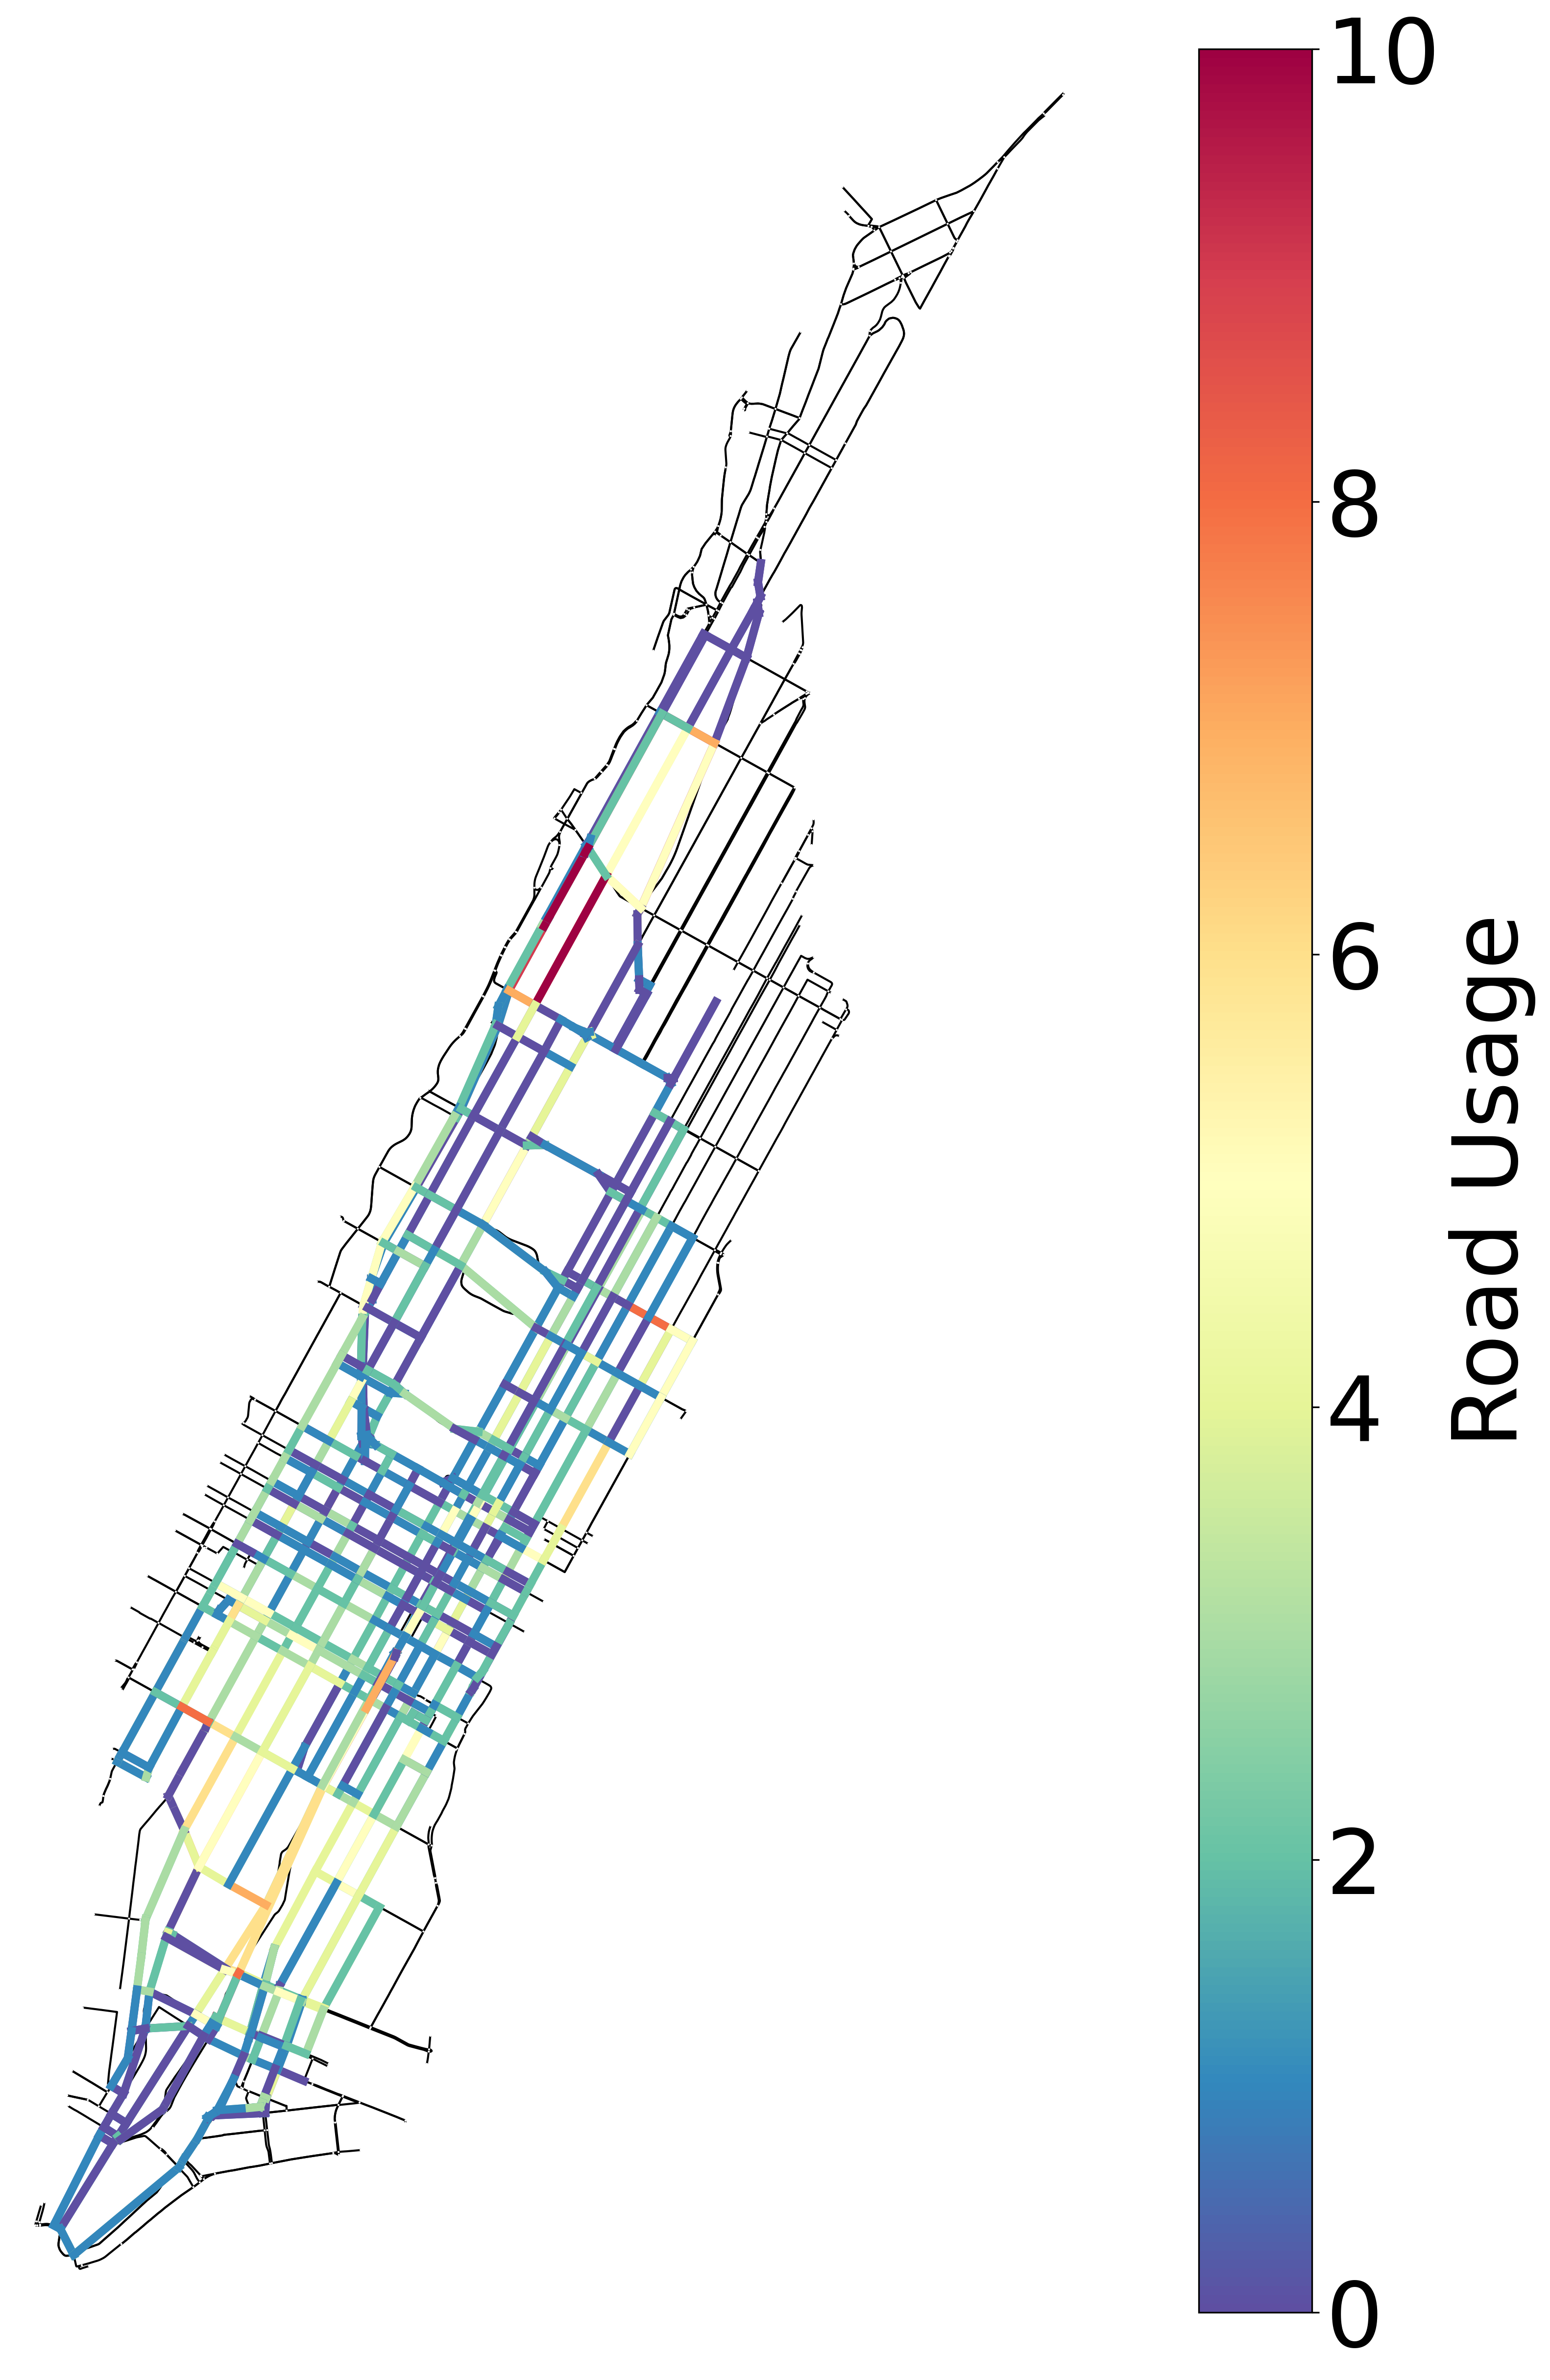
\includegraphics[width=\textwidth]{assets/img/07_graph_based/nyc_road_usage_simu_2.png}
		\caption{}
		\label{fig:nyc_road_usage_rebalancing_simu_2}
	\end{subfigure}
	\begin{subfigure}{0.5\textwidth}
		\begin{tikzpicture}
			\begin{axis}[
				xlabel={Iteration},
				ylabel={Charge (\%)},
				xtick={0,1,2,3,4,5,6,7,8,9,10},
				width=7cm,
				%legend pos=north west,
				legend style={at={(1.05,1)},anchor=north west},
				ymajorgrids=true,
				grid style=dashed,
				ytick = {20,40,60,80,100},
				thick,
				]
				
				\addplot[color = viridisbluecolor]
				coordinates {
					(0,100.0)
					(1,100.0)
					(2,100.0)
					(3,48.97903916555408)
					(4,15.884877155086665)
					(5,45.88487715508666)
					(6,73.0630622406528)
					(7,100.0)
					(8,100.0)
					(9,42.07152629790154)
				};
				\addplot[color = viridisyellowcolor]
				coordinates {
					(0,100.0)
					(1,100.0)
					(2,51.71688739117997)
					(3,53.63909930335382)
					(4,83.63909930335382)
					(5,100.0)
					(6,100.0)
					(7,100.0)
					(8,100.0)
					(9,100.0)
				};
				\addplot[color= viridisgreencolor]
				coordinates {
					(0,97.17818508556614)
					(1,100.0)
					(2,100.0)
					(3,100.0)
					(4,93.65529655770544)
					(5,100.0)
					(6,100.0)
					(7,100.0)
					(8,100.0)
					(9,67.45850236152518)
				};
				
				\addplot[color= viridisorangecolor]
				coordinates {
					(0,40.08880224745126)
					(1,70.08880224745127)
					(2,35.16396316489959)
					(3,56.5502211648996)
					(4,86.5502211648996)
					(5,100.0)
					(6,100.0)
					(7,93.0351864737918)
					(8,96.59822045507258)
					(9,96.59822045507258)
				};
				
				\addplot[ color = viridispurplecolor]
				coordinates {
					(0,15.921044602317869)
					(1,7.532559752269016)
					(2,32.02851575226901)
					(3,62.02851575226901)
					(4,92.02851575226902)
					(5,49.18398012599577)
					(6,79.18398012599576)
					(7,91.386258)
					(8,89.35404558665091)
					(9,91.386258)
				};
				
				\legend{2,6,7,9,18}
			\end{axis}
			
		\end{tikzpicture}
		\caption{}
		\label{fig:ex_soc_vehicles_rebalancing_simu_2}
	\end{subfigure}
	
	%\caption{Road Usage and State of Charge of an exemplary Set of Vehicles for the Simulation 2 with Rebalancing.}
	%\label{fig:ex_soc_rebalancing_simu_2}
%\end{figure}
%\begin{figure}[th]

	\begin{subfigure}[b]{0.35\textwidth}
		\centering
		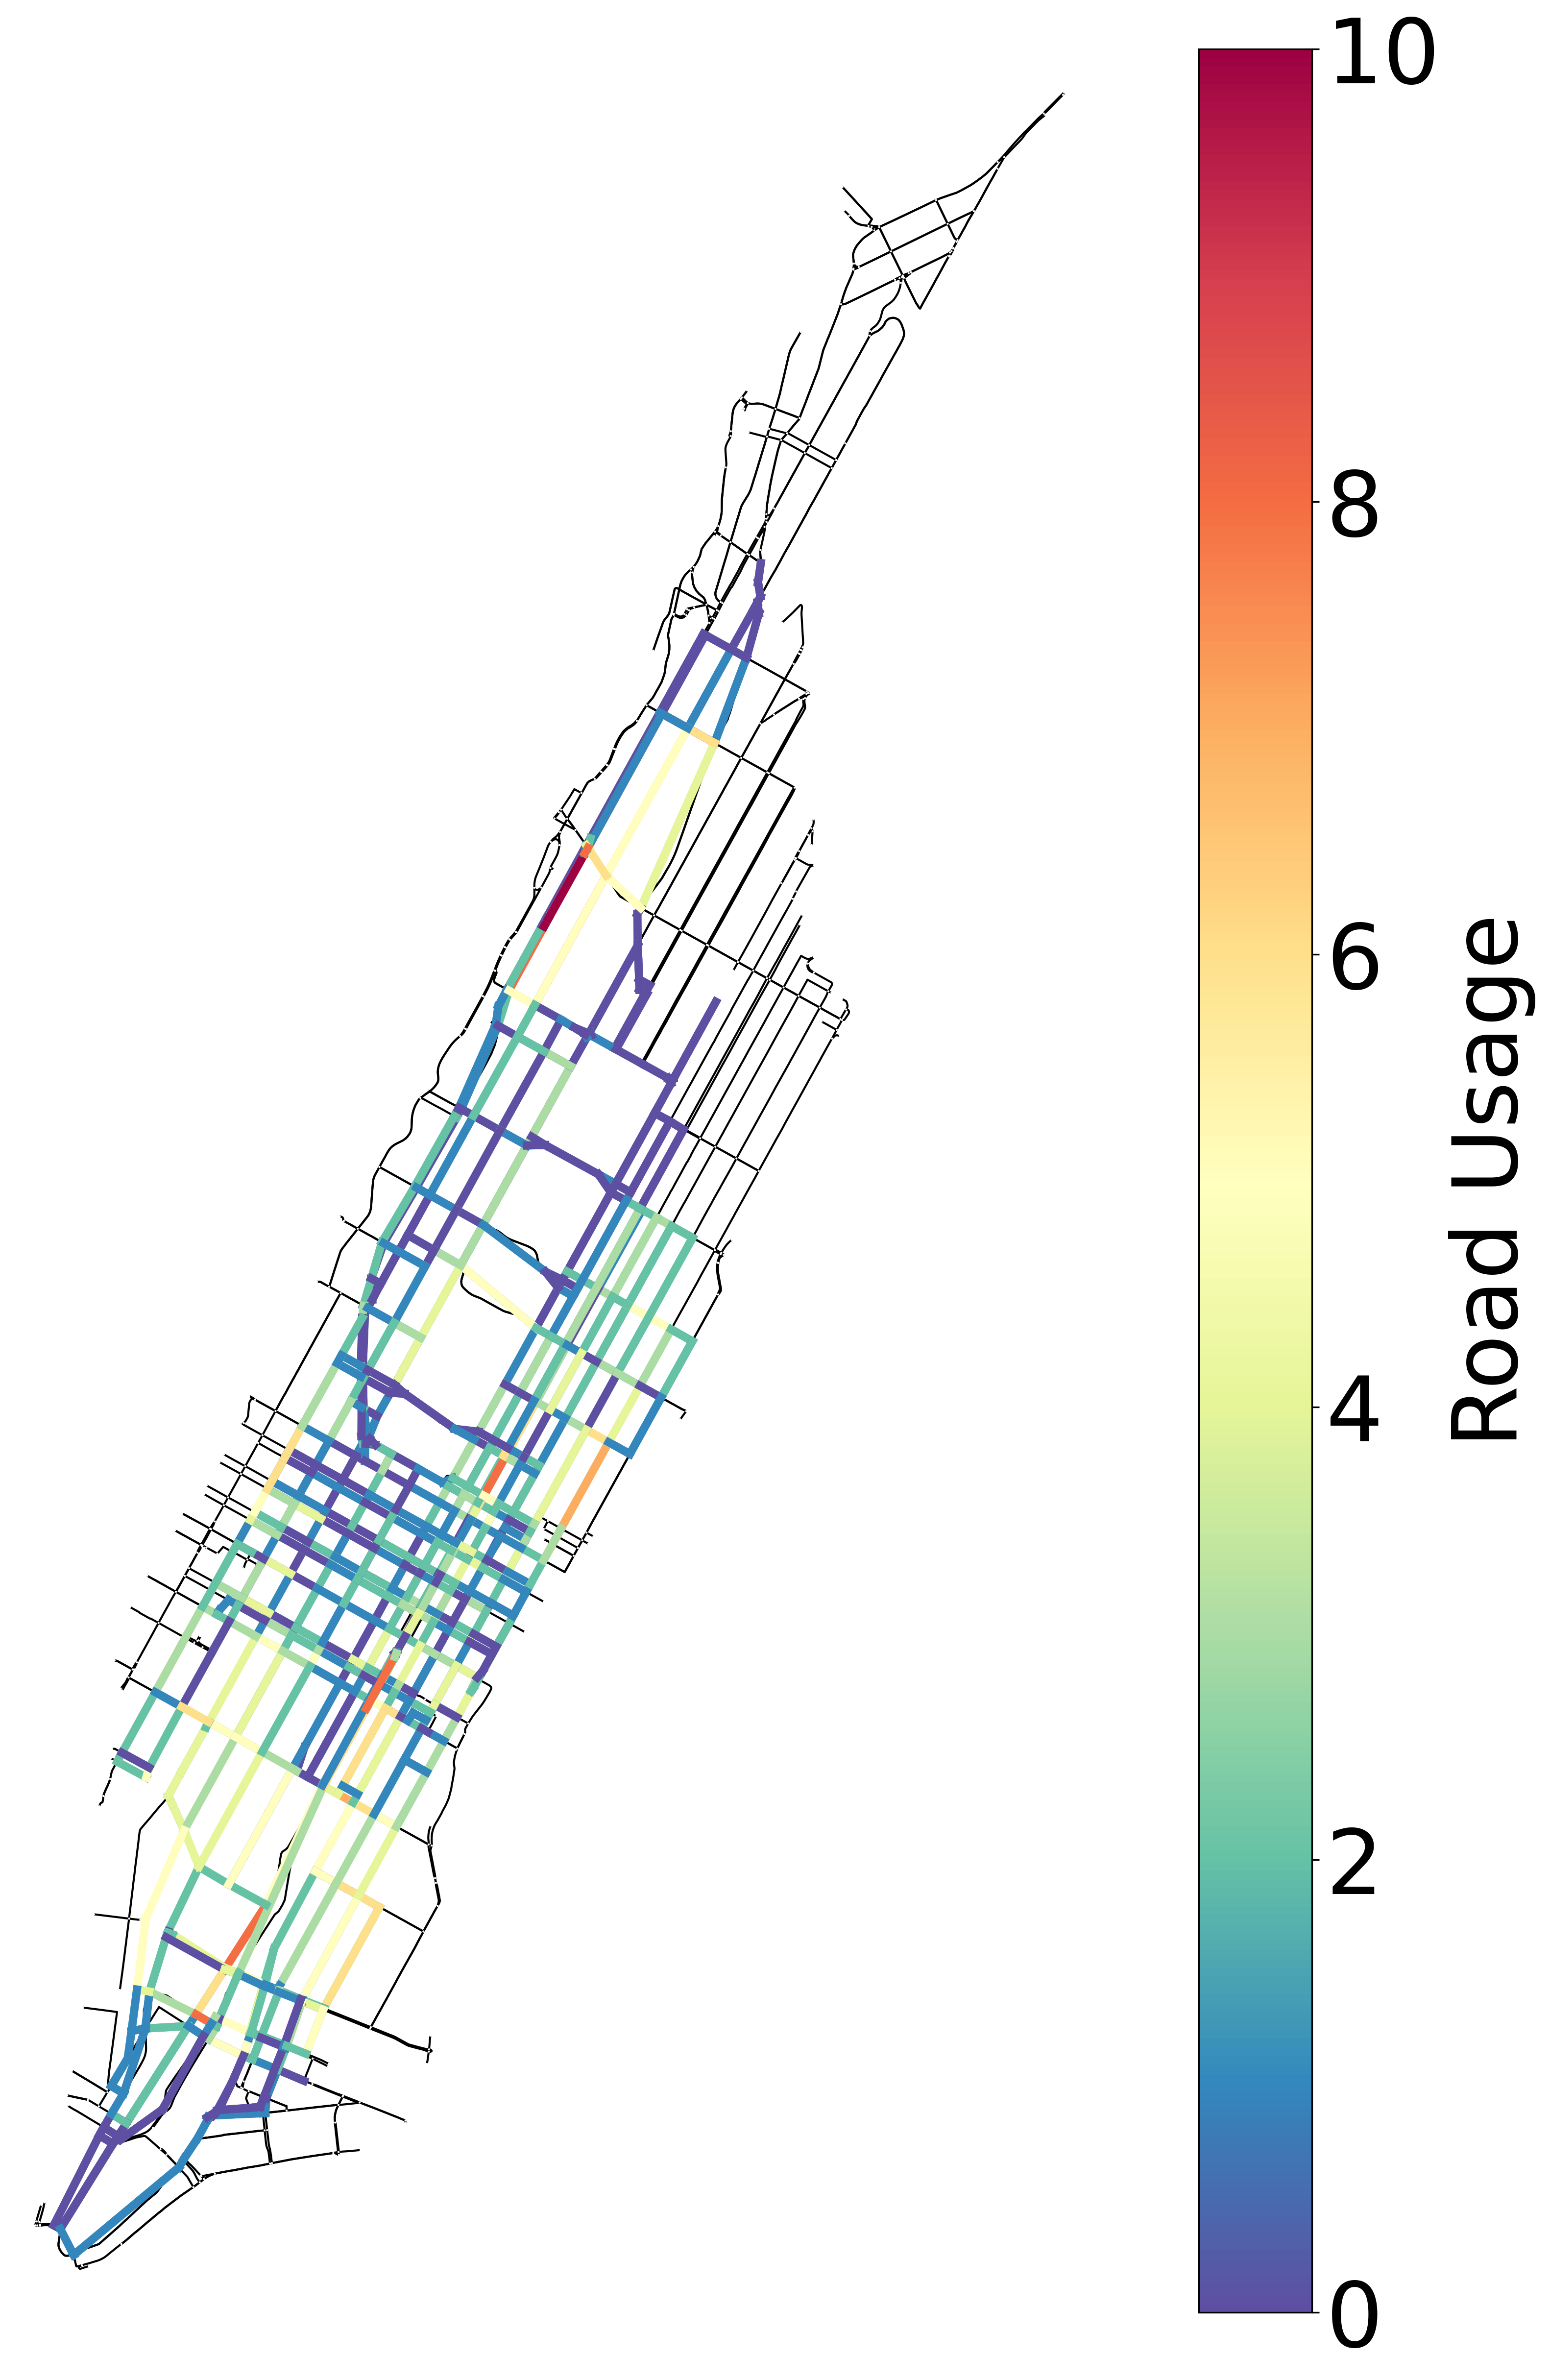
\includegraphics[width=\textwidth]{assets/img/07_graph_based/nyc_road_usage_simu_3.png}
		\caption{}
		\label{fig:nyc_road_usage_rebalancing_simu_3}
	\end{subfigure}
	\begin{subfigure}{0.5\textwidth}
		\begin{tikzpicture}
			\begin{axis}[
				xlabel={Iteration},
				ylabel={Charge (\%)},
				xtick={0,1,2,3,4,5,6,7,8,9,10},
				ytick = {20,40,60,80,100},
				width=7cm,
				%legend pos=north west,
				legend style={at={(1.05,1)},anchor=north west},
				ymajorgrids=true,
				grid style=dashed,
				thick,
				]
				
				\addplot[color = viridisbluecolor]
				coordinates {
					(0,91.87889400000002)
					(1,100.0)
					(2,72.0292442586887)
					(3,82.0292442586887)
					(4,92.0292442586887)
					(5,96.59822045507258)
					(6,67.12365203458644)
					(7,77.12365203458644)
					(8,87.12365203458644)
					(9,15.850743832355253)
				};
				\addplot[color = viridisyellowcolor]
				coordinates {
					((0,100.0)
					(1,100.0)
					(2,100.0)
					(3,41.1847448255528)
					(4,51.1847448255528)
					(5,27.621334976513168)
					(6,37.62133497651317)
					(7,47.62133497651317)
					(8,57.62133497651317)
					(9,59.57593497651317)
				};
				\addplot[color= viridisgreencolor]
				coordinates {
					(0,97.45850236152518)
					(1,93.70510142499876)
					(2,49.53183952806288)
					(3,13.35341540878908)
					(4,23.35341540878908)
					(5,33.35341540878908)
					(6,43.35341540878908)
					(7,53.35341540878908)
					(8,26.710786930371885)
					(9,29.12542616417984)
				};
				
				\addplot[color= viridisorangecolor]
				coordinates {
				(0,94.23546)
				(1,100.0)
				(2,93.8495732710165)
				(3,100.0)
				(4,100.0)
				(5,48.5010353935112)
				(6,58.5010353935112)
				(7,68.5010353935112)
				(8,78.5010353935112)
				(9,88.5010353935112)
				};
				
				\addplot[ color = viridispurplecolor]
				coordinates {
					(0,54.71009343582815)
					(1,64.71009343582816)
					(2,27.11306490355274)
					(3,37.11306490355274)
					(4,5.801929018188304)
					(5,15.801929018188304)
					(6,25.801929018188304)
					(7,35.801929018188304)
					(8,42.40014947326089)
					(9,48.57787418992616)
				};
				
				\legend{0,1,7,12,17}
			\end{axis}
			
		\end{tikzpicture}
		\caption{}
		\label{fig:ex_soc_vehicles_rebalancing_simu_3}
	\end{subfigure}
	
	%\caption{Road Usage and State of Charge of an exemplary Set of Vehicles for the Simulation 3 with Rebalancing.}
	%\label{fig:ex_soc_rebalancing_simu_3}
	\caption[Road Usage and State of Charge of an exemplary Set of Vehicles for the Simulation 2 and 3 with Rebalancing.]{Road Usage and State of Charge of an exemplary Set of Vehicles for the Simulation 2 and 3 with Rebalancing. \subfigref{fig:nyc_road_usage_rebalancing_simu_2} and 	\subfigref{fig:ex_soc_vehicles_rebalancing_simu_2} refer to Simulation 2, while \subfigref{fig:nyc_road_usage_rebalancing_simu_3} and 	\subfigref{fig:ex_soc_vehicles_rebalancing_simu_3} depict Simulation 3. }
	\label{fig:ex_soc_rebalancing_simu_2_3}
\end{figure}

\section{Conclusion}
This chapter demonstrated how an autonomous transportation system can be modeled, organized and evaluated in order to offer a better service to the customers. The dispatching, routing and rebalancing problems have been formulated and different versions have been proposed. Furthermore, a use case is demonstrated and a possible analysis has been proposed, with the goal of formulating considerations for a better fleet and road network usage. While this is to consider only as an example, multiple outcomes have been reached, which could be used to improve the quality of life of residents of traffic-cities cities such as NYC. Even if it focused on customer transportation and door-to-door delivery for urban cities, however, the analysis of a more bespoken model can be adapted for buisness logistics and transportation. Anticipated consequences included both negative effects, like heightened road and vehicle utilization due to rebalancing, and positive outcomes, such as improved service efficiency. However, unexpected outcomes, such as increased delivery demands with road capacity constraints, were also observed. The system, furthermore, can still be improved, as described in \secref{sec:mode_evaluation_ats} and observed in \secref{sec:use_case_analysis_ats}. The latter, specifically, highlited the need of a better cohesive strategy during the shift which would make optimal decision for the present also in regard of the future.\\
Despite this, the analysis serves as a foundational framework to inform decisions aimed at fostering a more sustainable and livable environment through optimized road usage and reduced vehicle emissions.



%\section{TO-DO}
%\begin{itemize}

%	\item Make the battery model in terms of the links. The time is, basically, the velocity of that link over the distance.
%	\item The time must be adapted according to the link travelling time. I.e., each request has a time window. The time from the inbound link must be within the time window.
%	\item Create a simulation using some fake data
%\end{itemize}
%\begin{itemize}
%	\item maybe use  a kalman filter to estimate requests per time
%\end{itemize}
